\documentclass[10pt,english]{report}
\usepackage[T1]{fontenc}
\usepackage[latin9]{inputenc}
\usepackage[a4paper]{geometry}
\geometry{verbose}
\pagestyle{plain}
\usepackage{babel}
\usepackage{csquotes}
\usepackage{graphicx}
\usepackage{amsmath}
\usepackage{setspace}
\onehalfspacing
\usepackage[unicode=true, pdfusetitle,
 bookmarks=true,bookmarksnumbered=false,bookmarksopen=false,
 breaklinks=false,pdfborder={0 0 1},backref=false,colorlinks=true,
 citecolor=black,filecolor=black,linkcolor=black,urlcolor=black]
 {hyperref}

\usepackage{fouriernc}
\usepackage{siunitx}
\usepackage{microtype}
\usepackage{nicefrac}

%\usepackage[colon,authoryear,sort&compress]{natbib}

\usepackage[natbib=true]{biblatex}
\bibliography{cpgs}

\usepackage{ccaption}
\captionwidth{5in}
\changecaptionwidth
\captionnamefont{\bfseries}

\begin{document}

\author{Gen Zhang\\
	Churchill College, Cambridge}
\title{Phenomenological approach to tissue maintenance and growth}

\maketitle

%\setlength{\parindent}{0pt} 
%setlength{\parskip}{1.4ex}

\pagenumbering{roman}

\begin{abstract}
\addcontentsline{toc}{chapter}{Abstract}
Abstract
\end{abstract}

\tableofcontents

\chapter{Introduction}
\setcounter{page}{1}
\pagenumbering{arabic}

Modern biochemistry has made enormous progress in understanding the laws governing life. We now know the framework by which cells undergo their business, we can sequence DNA and RNA at will, and are beginning to understand the complex interplay of those elements with proteins. This reductionist approach, ubiquitously successful elsewhere in science, promises much.

Nevertheless, just like full understanding of fundamental physics, \emph{ala} the Standard Model of particle physics, is unnecessary for understanding properties of superconductors, we would argue that the wealth of biochemical information may be distilled into simple models. Indeed, such a distillation may be necessary, for two reasons. One is what we would do if we had exact knowledge of all biochemical pathways in cellular processes, including the ability to understand protein expression; even in a given cell, the number and speed of such chemical reactions would lead to models with such bewildering complexity that even if we were able to solve them, we would hardly \emph{understand} better the system --- ``comprehension is compression'' \citep{chaitin2002intelligibility}. Two is that new laws can emerge from collective phenomenon; just like superconductivity has nothing to do with a single electron, or even a handful, it may be that at the tissue level, the dominant phenomena are emergent behaviours of a macroscopic number of cells.

In recent years, we have seen the raise in popularity in so-called ``systems biology'', where one tries to measure as much quantitative data as possible (gene expressions, chemical concentrations and gradients, etc.) and incorporate such data with mathematical models which attempt to account for as much of known interactions and interrelations as possible. From this point, macroscopic characteristics such as functional states of the cells and even tissue may be quantitatively understood. This has been especially successful in systems where the relevant system components can be identified with ease, such as in prokaryotes or simple single-celled eukaryotes [??]. However, in truly multi-cellular tissue, the possible interactions and cell fate are potentially much more complex.

We thus promote a phenomenological approach, where a theory is sought which directly relate measurable macroscopic quantities, motivated by obvious constraints such as spatial homogeneity or existence of robust long-term physiological function. Such models are justified solely by their predictive ability, and can assist in identifying the relevant microscopic components, which may then be used in a fuller theory.

Such an approach has enjoyed great success in traditional condensed matter, culminating in the great Landau theory of equilibrium phase transitions, and the understanding of ``universality'', where wildly different microscopic systems nevertheless shared exact quantitative behaviours. Such approaches have also been pushed to study non-equilibrium systems \citet[chapter 10]{cardybook}, and have revealed a consistent and richer landscape. There is nothing special about biological tissue which precludes such an approach.

We are aided by the recent availability of experimental techniques capable of tracking tissue growth with cellular resolution. In particular, inducible genetic labelling gives access to \emph{full counting statistics} which are not even available in traditional condensed matter systems. In addition, it may be possible to truly measure two point correlations, in both time and space. Such wealth of experimental data are unimaginable with electrons, phonons, etc., and as such may provide fertile testing ground for well developed theories which has so far lacked the necessary experimental verification.

\paragraph{Outline of research}

In chapter \ref{ch:oes} we study a model tissue of squamous stratified epithelium: mice oesophagus. It is a continuation of the work in \citet{clayton,klein07}. The availability of full counting statistics (as opposed to just statistics of the basal layer) allows us unprecedented power in resolving cell fate. This ability is then applied to further understand cell cycle, drug treatment and scrutinise a suggestion of a discrete sub-population of stem cells.

In chapter \ref{ch:voter} we begin exploring the phenomenological theories of non-equilibrium which obey the tight constraints of spatial homogeneity and tissue homoeostasis.

In chapter \ref{ch:spinal-chord} we present some preliminary work on a system far from homoeostasis: the development of spinal chord in chick embryo. The existence of precise counts of cells at each stage of development provides strong constraints when considering models of cell fate choice.

We conclude with a discussion of open questions and potential future work in chapter \ref{ch:conclusion}.

\chapter{\label{ch:oes}Parameters of epithelial maintenance}

This work has been carried out in collaboration with Phil Jones and David Doup\'e at MCR Hutchinson, Cambridge.

\section{Introduction}

The oesophagus is lined with stratified squamous epithelium. That is, it consists of layers of keratinocytes and appears flat and featureless. It is a simple tissue which undergoes constant renewal through adult life. Structurally, it is almost identical to the mammalian interfollicular epidermis considered by \citet{clayton}, so it is a good model tissue for understanding cell fate choice and tissue maintenance.

Proliferation in the oesophageal epithelium is confined to cells in the basal layer \citep{leblond}. These proliferating cells may commit to terminal differentiation and exit the cell cycle, and migrate (stratify) into the first suprabasal layer. They then undergo dramatic changes whilst continuing migration upwards, which eventually result in their loss by shedding at the surface \citep{seery}.

\begin{figure}[h]
	\centering
	\includegraphics[width=4in]{oesophagus-anatomy.png}
\end{figure}

\citet{klein07} introduced a non-equilibrium model for the homoeostatic maintenance, based around a single population of \emph{committed progenitors} (CP) cells:

\begin{figure}[h]
	\centering
	\includegraphics[width=4in]{oesophagus-division-process.png}
\end{figure}

Cell division, stratification and fate choice are assumed to be stochastic and independent. Such a process falls into the well-studied class of \emph{branching processes} \citep{athreya&ney}, and are known to be tractable. The three parameters $\lambda$, $\gamma$ and $r$ are the only parameters of the system and for a given initial condition completely determine subsequent evolution by the master equation:
\begin{align}
\nonumber
\frac{dP_{m,n,l}}{dt} &= \lambda\left[r (m-1)P_{m-1,n,l} + (1-2r)mP_{m,n-1,l} + r(m+1)P_{m+1,n-2,l} - mP_{m,n,l}\right] \\
                    &+ \gamma\left[(n+1)P_{m,n+1,l-1} - nP_{m,n,l}\right] \label{eq:ABC-master} \\
\nonumber
P_{m,n,l}(t = 0) &= \delta_{m,1} \delta_{n,0} \delta_{l,0}
\end{align}
where $P_{m,n,l}$ are the probabilities of seeing a clone with $m$ committed progenitors, $n$ terminally differentiated cells in the basal layer, and $l$ suprabasal cells. For homoeostasis, the proportion $\rho$ of CP cells in the basal layer must obey
\begin{equation}
\rho \lambda = (1-\rho) \gamma.\label{eq:homoeostatic-rho}
\end{equation}
In fact, for any initial condition the actual proportion will converge to this homoeostatic value.

Experimentally, a representative population of progenitor cells are labelled with an inducible genetic marker expressing the enhanced yellow fluorescent protein (EYFP) gene. Induction proceeds via drug (tamoxifen) treatment and, importantly, may be kept to a low frequency, such that individual clones may be resolved with confidence. Whilst shedding of suprabasal cells in a clone are not significant, it is possible to collect statistics of the number of basal and suprabasal cells in each clone. At longer times, suprabasal counts are not reliable, but basal statistics are still accessible.

It is then a simple matter of inference to extract from the experimental data the parameters $\lambda$, $\rho$ and $r$, and thus by equation \eqref{eq:homoeostatic-rho} the stratification rate $\gamma$. In section \ref{sec:ki67}, comparing the parameters obtained this way against the methodology used in \citet{clayton}, we find some discrepancies and come to the conclusion that the oft-used proliferation marker Ki67 is in fact not tight, and fail to label some cells still in cycle. Intriguingly, it is found that $\rho \simeq 1/2$, suggesting that stratification and division may be linked.

Against this back drop of quantitative measurements of cell fate, the effect of drug treatment with \emph{all-trans retinoic acid} (ATRA) is characterised in section \ref{sec:atra}. We find that the only effect is an increase of division rate $\lambda$, with a proportional response in $\gamma$, such that $\rho$ is kept constant. This is enough to explain all the clonal data, without invoking potentially non-equilibrium transient behaviour. In particular, it side-steps the confounding complications that hampered the analysis in \citet[][chapter 4]{kleinthesis}.

In section \ref{sec:oesophagus-stem} we investigate the claim that there is a discrete population of stem cells \citep{kabalis}, and find some support in the anomalous proportions of single cell clones. However, they are largely quiescent and make negligible contributions to homoeostatic maintenance.

\section{\label{sec:oesophagus-scaling}Scaling in theory and practice}

\citet{klein07} and \citet{tediousharvard} made extremely detailed studies of equation \eqref{eq:ABC-master}; more specifically, they studied the reduced two-type process where stratified cells were not counted, i.e.\ only basal clonal statistics were considered. They showed that this model exhibits scaling, where in the large time limit $t\rightarrow\infty$ the clone size distribution becomes exponential: $$P^\textrm{surv.}_n \sim \exp\left(-\frac{n}{\left\langle n^\textrm{surv.} \right\rangle}\right)$$ with a linear growth of the average size of surviving clones $\left\langle n^\textrm{surv.} \right\rangle \rightarrow t/\tau$ and characteristic time scale $\tau = \rho/r\lambda$. This can be shown by noting that large clones are macroscopic, and fluctuations in the proportion of CP cells versus differentiated cells are small --- in essence large clones are overwhelmingly likely to be representative of the tissue as a whole. \citealt{tediousharvard} have shown that this process happens remarkably quickly, and clones of even ten cells become quite representative. Thus, we can erase the difference between CP and differentiated cells, and average them into a \emph{representative basal cell} obeying extremely simple dynamics: 

\begin{figure}[h]
	\centering
	\includegraphics[width=3in]{oesophagus-average-division-process.png}
\end{figure}

This is now a classic \emph{one-type critical branching process} \citep{athreya&ney}, and has an exact solution. The clone size distribution is geometric at all times $$P^\textrm{surv.}_n \sim \left(1-\frac{1}{\left\langle n^\textrm{surv.} \right\rangle}\right)^n$$ with an average clone size $\left\langle n^\textrm{surv.} \right\rangle = 1 + t/\tau$. Confirmation of this scaling behaviour in \citet{clayton} lead to the overturning of the previously incumbent stem/transit amplifying model \citep{stemta1,stemta2,stemta3}, in favour of the current single progenitor model.

\begin{figure}[htb]
	\centering
	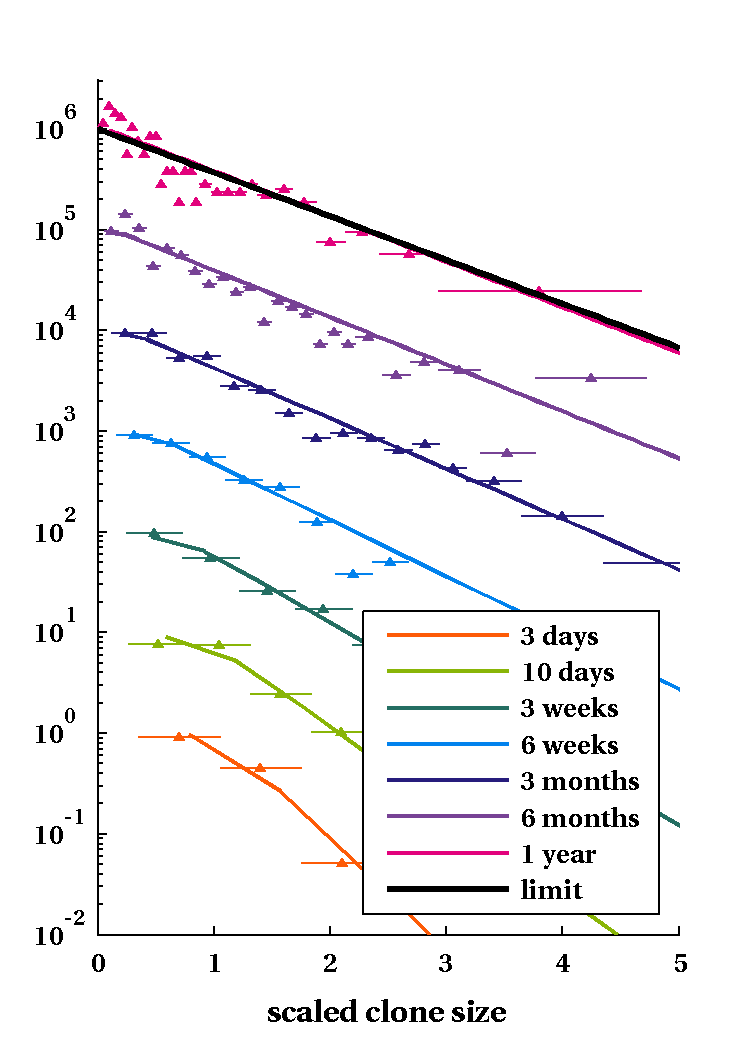
\includegraphics[width=3in]{oes-scaling-b.png}
	\caption{The basal clone size distribution displays the expected scaling behaviour, converging to an exponential.}
\end{figure}


Although theoretically very attractive, this long-time scaling behaviour is actually unhelpful in so far as inferring the parameters from experimental data. Since after just a few cell divisions the clone distribution becomes a featureless exponential, it is only possible to measure the characteristic time scale $\tau$ (though, as we shall see, this may be determined very accurately). The separate constituents of $\tau$ have to be measured by something other than clonal statistics: the division rate $\lambda$ may be directly measured from observation of proliferation; the proportion of proliferating progenitor cells $\rho$ may be measured from the expression of the genetic marker Ki67; and $r$ may be obtained by inverting the equation $\tau = \rho/r\lambda$. However, these all introduce additional errors, both systematic and random; worse, these errors are difficult to estimate. In particular, if the genetic marker is unreliable or inefficient (see section \ref{sec:ki67}), then this would have a very direct effect on the inferred value of $r$.

To do better, it is necessary concentrate on the short-time behaviour and the approach to scaling. In particular, unlike \citet{clayton} we have access to the number of suprabasal cells in each clone, \emph{at a only a few division times}. This compels us to use a fully Bayesian method.

\section{Practicalities of Bayesian inference}

To apply a Bayesian method, we need a prior distribution for the parameters, and a likelihood function for seeing a particular outcome for a particular set of parameters. Without further biological motivation, a maximum entropy prior was chosen in $(\lambda, \rho, r)$-space: log-uniform in $\lambda$, uniform in $\rho$ and $r$. 

At first blush, equation \eqref{eq:ABC-master} is sufficient to calculate the likelihood function. However, it is an infinite set of coupled differential equations, for practical computation we must truncate it. In the case that we are examining data involving both basal and suprabasal counts, we can use a special structure of the master equation; namely, $\dot{P}_{m,n,l}$ only depends on $P_{a,b,c}$ for $a+b+c \le m+n+l$. Our data must have a maximum clone size, and so to find the theoretical prediction is is sufficient to truncate the probabilities to only include those of a smaller or equal size. After such a truncation, it is of the form $$\frac{d\mathbf{P}}{dt} = \mathbf{TP}$$ where the transition matrix $\mathbf{T}$ is sparse. The exact solution is then $$\mathbf{P}(t) = \exp\left(\mathbf{T}t\right) \mathbf{P}_0,$$ and the matrix exponential may be taken with well-known methods using Krylov subspace techniques \citep{expokit}.

The case of only basal statistics is more involved. Because the observation does not look at the number of suprabasal cells, we effectively have an infinite sum over the index $l$, and no truncation would be accurate. Instead, we use a method inspired by \citet{tediousharvard} based on generating functions. The reduced probability distribution for just the basal cells is
\begin{align}
\tilde{P}_{m,n} &= \sum_l P_{m,n,l}, \nonumber \\
\frac{d\tilde{P}_{m,n}}{dt} &= \lambda\left[r (m-1)\tilde{P}_{m-1,n} + (1-2r)m\tilde{P}_{m,n-1} + r(m+1)\tilde{P}_{m+1,n-2} - m\tilde{P}_{m,n}\right] - \gamma n \tilde{P}_{m,n}, \label{eq:AB-master} 
\end{align}
and upon applying some generatingfunctionology
\begin{align}
f(x,y,t) &= \sum_{m,n} x^m y^n \tilde{P}_{m,n}(t), \nonumber \\
f_t &= \lambda \left[ r x^2 + (1-2r) xy + r y^2 - x \right] f_x - \gamma y f_y, \label{eq:AB-gf}\\
f(x,y,t=0) &= x. \nonumber
\end{align}
The partial differential equation for $f(x,y,t)$ may be solved by the method of characteristics, which converts it into a single (non-linear) ordinary differential equation in one variable; this may then be numerically integrated. Since we cannot distinguish between progenitors and cells committed to terminal differentiating, we actually care about the single variable generating function 
\begin{equation*}
g(z,t) = f(z,z,t) = \sum_k z^k \sum_{m+n=k} \tilde{P}_{m,n}(t).
\end{equation*} 
Noting $g(z,t)$ is a power series in $z$ and $g(z=1,t) = 1$ by conservation of probability, it must be the case that $g(z,t)$ converges at least on the (open) unit disc. Making the assumption that it actually converges on the closed unit disc in the complex plane, we are led to the inversion formula:
\begin{align}
\Pi_k(t) = \sum_{m+n=k} \tilde{P}_{m,n}(t) &= \frac{1}{2\pi i} \oint_\mathcal{C} \frac{g(z,t)}{z^{k+1}} dz \label{eq:cauchy-coefficients} \\
	&\simeq \frac{1}{N} \sum_{j=0}^{N-1} g\left[\exp\left(\frac{2\pi ij}{N}\right),t\right] \exp\left(\frac{2\pi ijk}{N}\right) \label{eq:fft-coefficients}
\end{align}
where the contour $\mathcal{C}$ goes counterclockwise about the origin in the complex $z$ plane. Taking it to be the unit circle, the approximation by a sum \eqref{eq:fft-coefficients} amounts to a discrete Fourier transform, which then allows the first $N$ coefficients to be computed efficiently with only $N$ evaluation of the generating function $g(z,t)$. In practice, some adaptive oversampling is used to make guarantees on numerical accuracy.

We note in passing that some information about the distribution $\Pi_k$ may be directly gleaned from the analytic properties of $g(z)$. In particular, since the ratio of successive terms $\Pi_{k} / \Pi_{k+1}$ converges to the radius of convergence of $g(z)$, it is possible to infer an exponential tail for $\Pi_k$ from the existence of singularities at a finite $\left| z \right|$, and indeed obtain the slope. It is interesting to ask what other properties may be so easily obtained; for example, whether a Gaussian tail (i.e.\ $\Pi_{k} / \Pi_{k+1} \sim k$) can be obtained `by inspection', and generally if such properties can be more directly obtained from considering the differential equation governing the generating function (e.g.\ equation \eqref{eq:AB-gf}) without having to explicitly find the solution.

\section{\label{sec:ki67}Ki67 is not a good marker}

Armed then with the necessary tools, it is a straightforward matter to apply Bayes' theorem and obtain posterior distributions for a given data set. Indeed, it is possible to apply this method to various different datasets, and thus gain some confidence in self-consistency. Figure \ref{fig:oes-inference-result} shows the results from both full counting statistics (basal and suprabasal counts) and only basal statistics (but over a much longer time period, with higher counts).

\begin{figure}[htb]
	\centering
	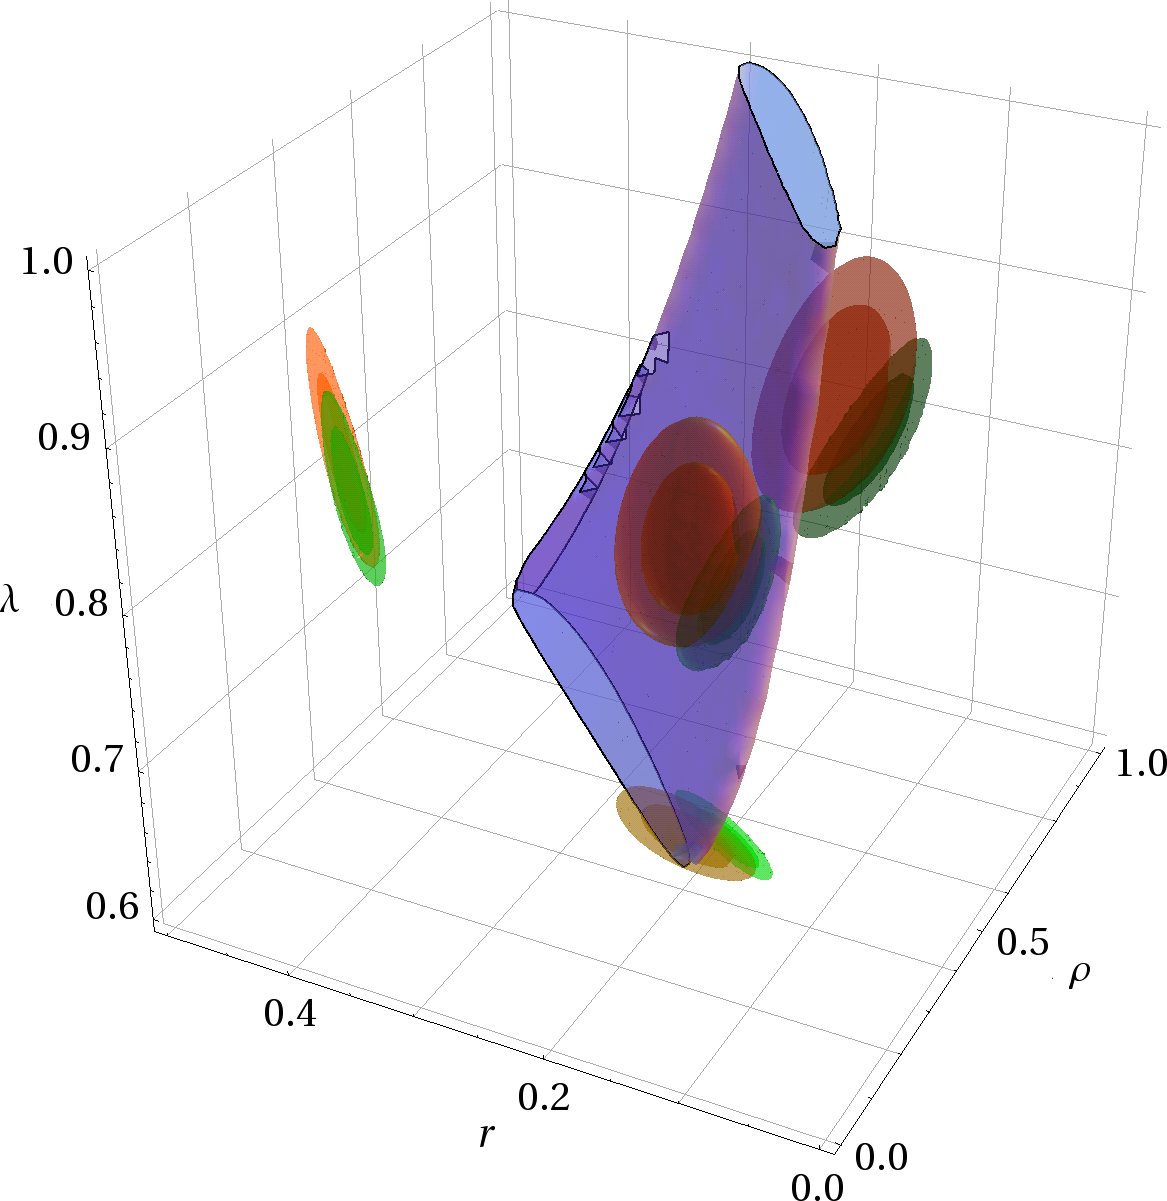
\includegraphics[height=3in]{oes-combined-prior.png}
	\caption{\label{fig:oes-inference-result}The inference from short time full counting data is in orange, showing $68\%$ and $95\%$ confidence regions. The inference from long time basal data is show in blue. The combined data produces the region (68\% and $95\%$) shown in green, with projections shown on the axes planes. The mean lies at $\rho = 0.52 \pm 0.07$, $r = 0.19 \pm 0.04$, $\lambda = (0.77 \pm 0.05) /\textrm{week}^{-1}$.}
\end{figure}

Using Ki67 to stain for progenitors, it was estimated $\rho \simeq 0.4$. It is discrepant with the clonal inference result $\rho = 0.52 \pm 0.07$. We suggest that the differences are due to a difference of what proliferation means. Ki67 is expressed during ribosomal RNA transcription \citep{ki67rRNA}, so measurements based on it are essentially measures of rRNA activity. Our methodology here more directly measures proliferation by potential cell division, purely on cell fate. The two can be reconciled if we postulate that there is a period of the cell cycle where rRNA activity ceases, before re-activating if the cell decides to remain in cycle. This point of view is further supported by companion studies in mice ear epidermis, where the cell cycle time is much longer at $\sim 4~\textrm{weeks}$; there, the Ki67 expression rate is around $\rho \simeq 0.24$, but clonal fate inference gives again $\rho \simeq 0.50$. This larger discrepancy can then be assigned to the increased cell cycle time, presumably lengthening the period when rRNA activity is quiescent.

\section{\label{sec:atra}The effects of ATRA, quantitatively}

In evaluating drug treatment, it is desirable to be able to be able to quantify the effects on the cellular level, as well as the overall phenotype changes. Conventional histology is unable to measure with precision the changes to cell proliferation rate or differentiation rate, or fate choices. With the base model that we have developed above, it is natural to ask if we can do better. As a prototypic drug, we studied the effects of \emph{all-trans retinoic acid} (ATRA) It is observed that in epidermis, ATRA leads to a new homoeostatic state, with increased suprabasal thickness, but no qualitative changes in the division process \citep{atraqualitative}. Under the assumption that oesophagus is structurally identical, we consider two experiments:

\begin{enumerate}
\item inducible genetic labelling after a few weeks of treatment with ATRA; full clonal statistics then characterise the new homoeostatic state;
\item begin ATRA treatment after labelling; clonal statistics reflect the transient behaviour in switching from one state to another.
\end{enumerate}

Crucially since the overall cell division process is conserved, and homoeostasis is retained, it is possible to apply the Bayesian inference framework already developed to the homoeostatic data, and directly measure the changes in the parameters of the division process. Doing so, we obtain $\rho = 0.5$, $r = 0.22$ and $\lambda = 1.4/\textrm{week}^{-1}$; i.e.\ the only significant changes are an increase in cell division rate, and a proportional change in cell stratification rate. This lends strong support that the two processes are actually locked together via some form of signalling, biochemical or physical (e.g.\ elastic stresses).

\citet[][chapter 4]{kleinthesis} considers a similar experimental set up in mouse tail epidermis. There, it is observed that a three-fold increase of $\rho$, as measured by Ki67 expression, occurs (increase from $19\%$ to $57\pm4\%$). With our current view on the role of Ki67 in the cell cycle (see section \ref{sec:ki67}), our interpretation is that the shortened cell cycle reduces the rRNA quiescent period, and thus boosts the Ki67 expression \emph{without changing the progenitor proportion}. In particular, this allows us to sidestep the complex theory of non-equilibrium transition between homoeostatic states considered by \citet{kleinthesis}. Instead, we can simply use the existing inference framework to effectively ask the question: what stage (i.e.\ number of mean cell cycle time) does this data set correspond to? This works equally well for wild-type (non-ATARA-treated), ATRA-homoeostasis and introduction of ATRA post-labelling. We find consistency with a model where ATRA increases cell cycle rate immediately to a new value, corresponding to the ATRA-homoeostatic rate.

Figure \ref{fig:oes-atra} show that the model accurately predicts the observed clonal size distribution.

\begin{figure}[htb]
	\centering
	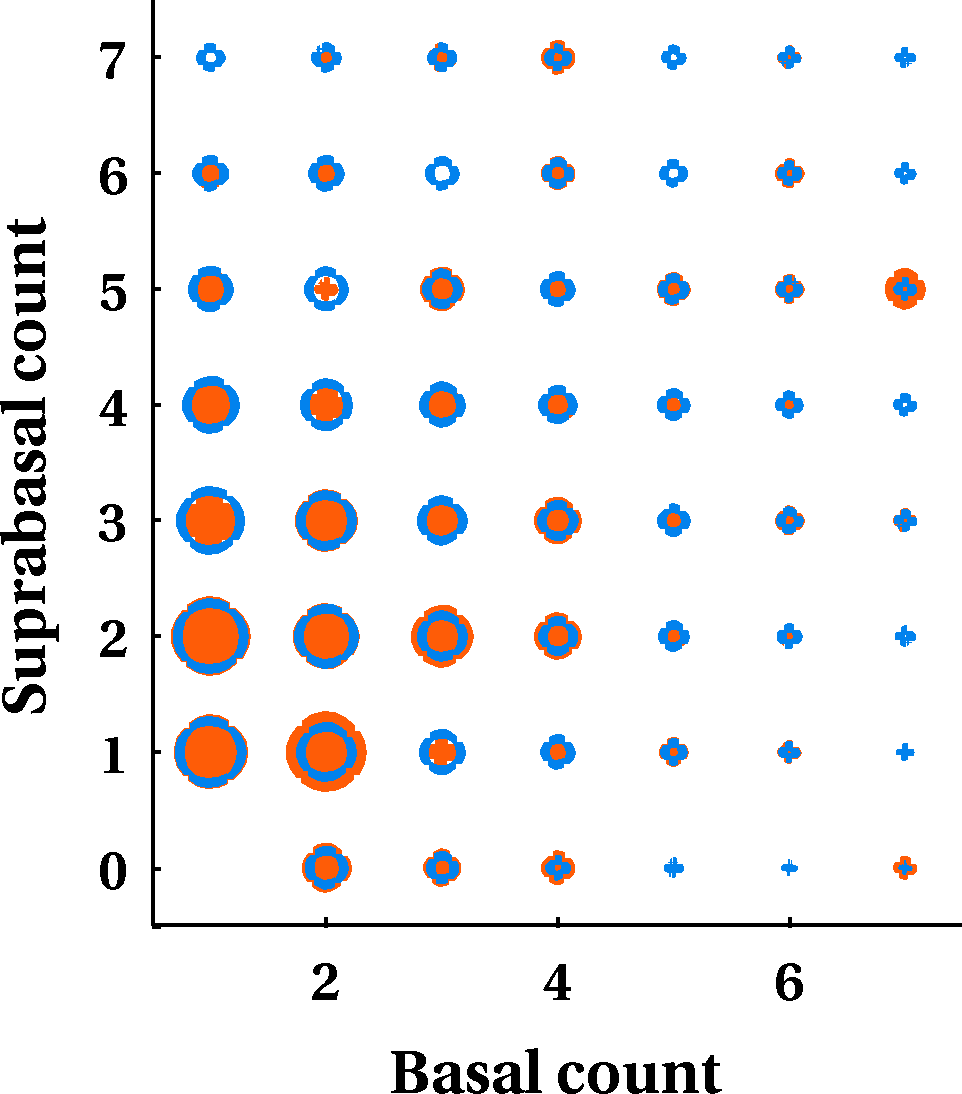
\includegraphics[height=2in]{oes-atra-bubbles.png}
	\caption{\label{fig:oes-atra}Orange filled circles show the observed clonal size distribution for ATRA pre-treated tissue, $3$ weeks after induction; blue dashed circles show the theoretical predictions. Deviations are well contained by stochastic noise and uncertainty in model parameters.}
\end{figure}

\section{\label{sec:oesophagus-stem}Stem cells in the oesophagus}

A recent study \citep{kabalis} has identified a sub-population of basal cells in oesophageal epithelium which are almost quiescent in normal homoeostasis, capable of reconstituting the epithelium in cultures and contribute cells to repair injured epithelium \emph{in vivo}; thus, they fulfil a functional definition of stem cells. At first glance, their quiescence in homoeostasis preclude our methodology so far from identifying them ore characterising them. Upon closer inspection however, if any of them get labelled, there would be a slight change of the clonal distribution, in the form of a population whose average size did not grow with time (or at least with a significantly different time scale).

We were then led to look closely at single cell basal clones, i.e. those with one basal cell, and no suprabasal cells at all. Suppose that stem cells undergo (near) balanced division into stem cells and committed progenitors; further, assume that $\lambda = \gamma$, i.e. $\rho=1$ exactly, we can then write time evolution of single cell clones (might be stem, might be progenitor/post-mitotic):
\begin{equation}
p_\textrm{single} = \rho_S \exp(-\Lambda t) + (1-\rho_S) \exp(\lambda t),
\label{eq:single-cell-clones}
\end{equation}
where $\rho_S$ is the proportion of labelled cells which are stem cells, and $\Lambda$ is the division rate of those stem cells. Note that although stem cells are likely be highly responsive to environmental effects (such as local density fluctuations) and thus not stochastic in the main, in homoeostasis we can effective average over such local fluctuations, and approximate their statistical behaviour as stochastic. Setting $\lambda = 0.76/\textrm{week}^{-1}$ (see section \ref{sec:ki67}), we can use a Bayesian method to infer the parameters $\Lambda$ and $\rho_S$; again, in the absence of more cogent biological constraints, we employ a maximum entropy prior: uniform in $\rho_S$, log-uniform in $\Lambda$.

\begin{figure}[htb]
	\centering
	\hfill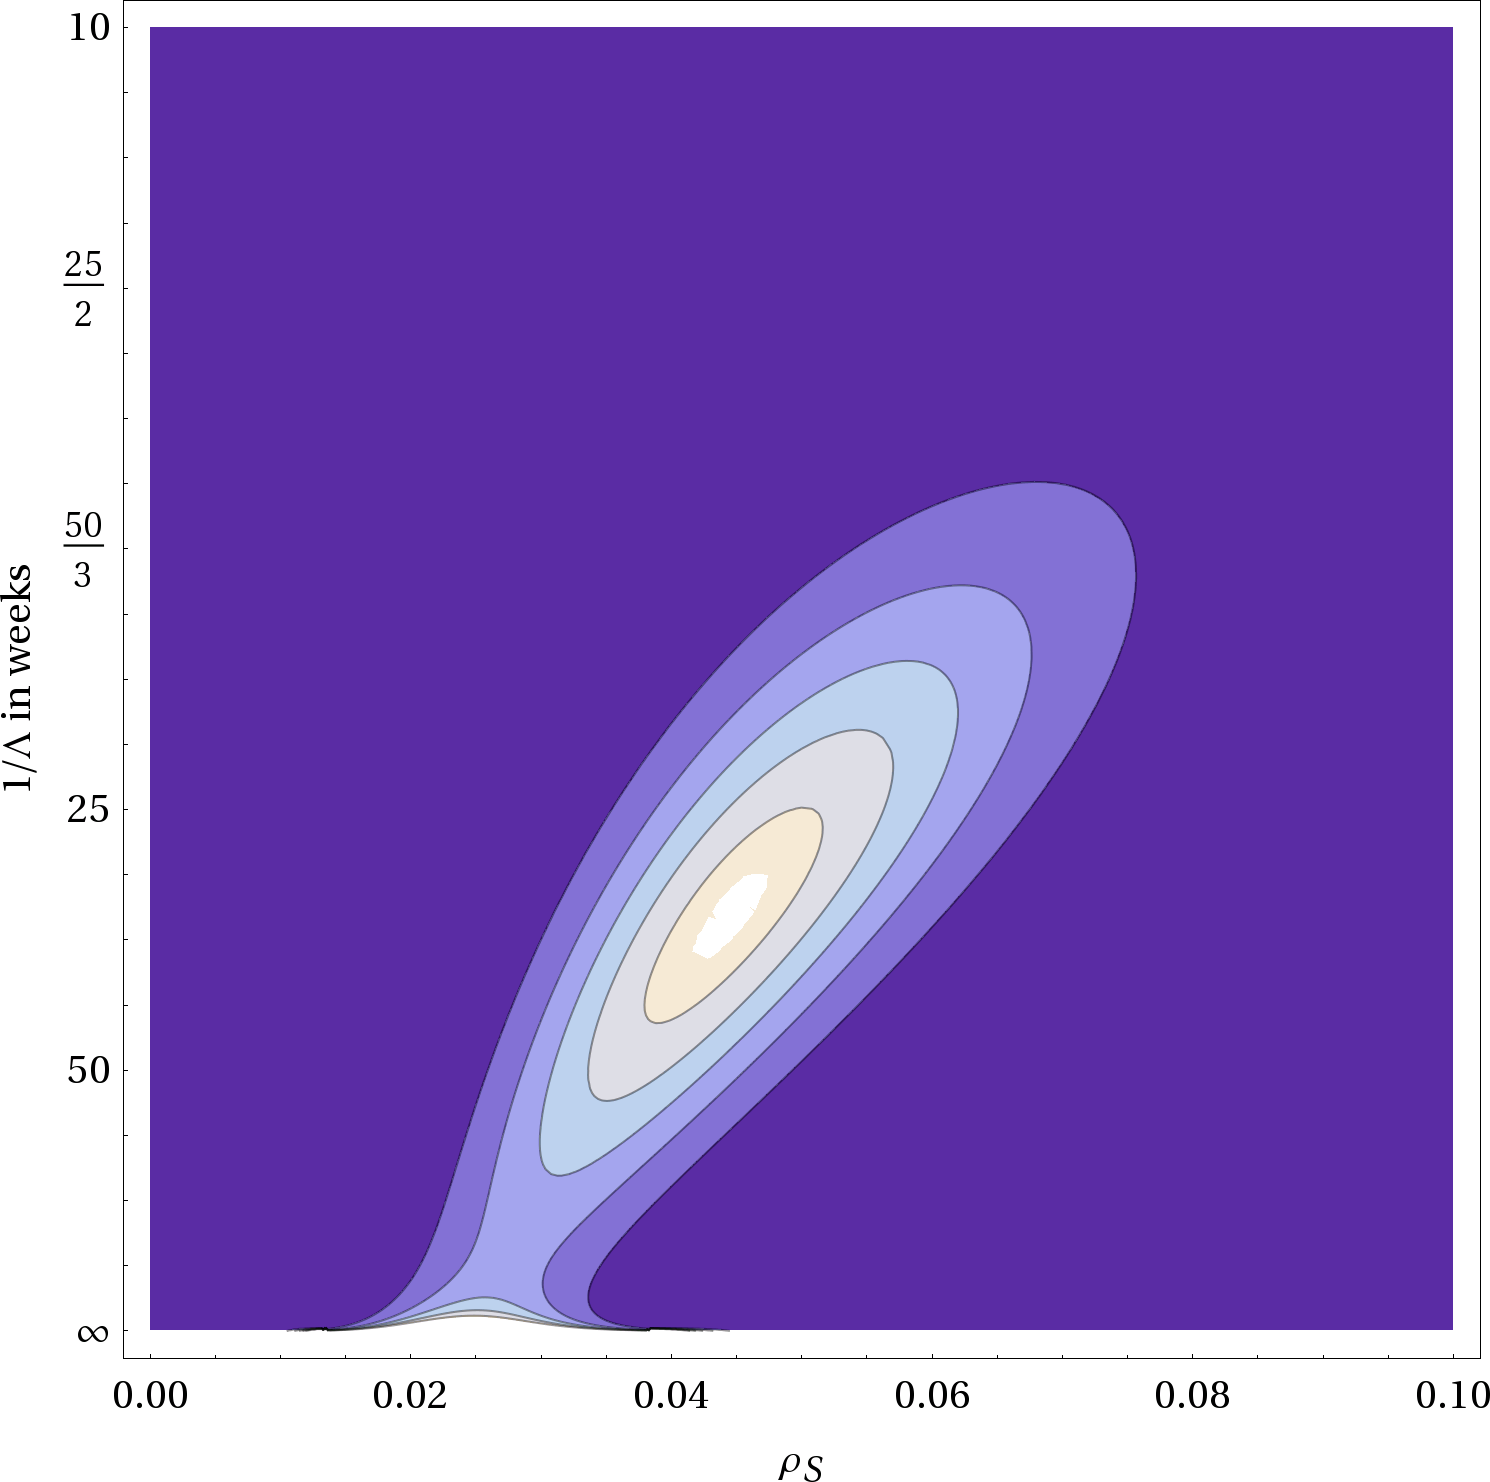
\includegraphics[height=2in]{single-cell-inference.png}\hfill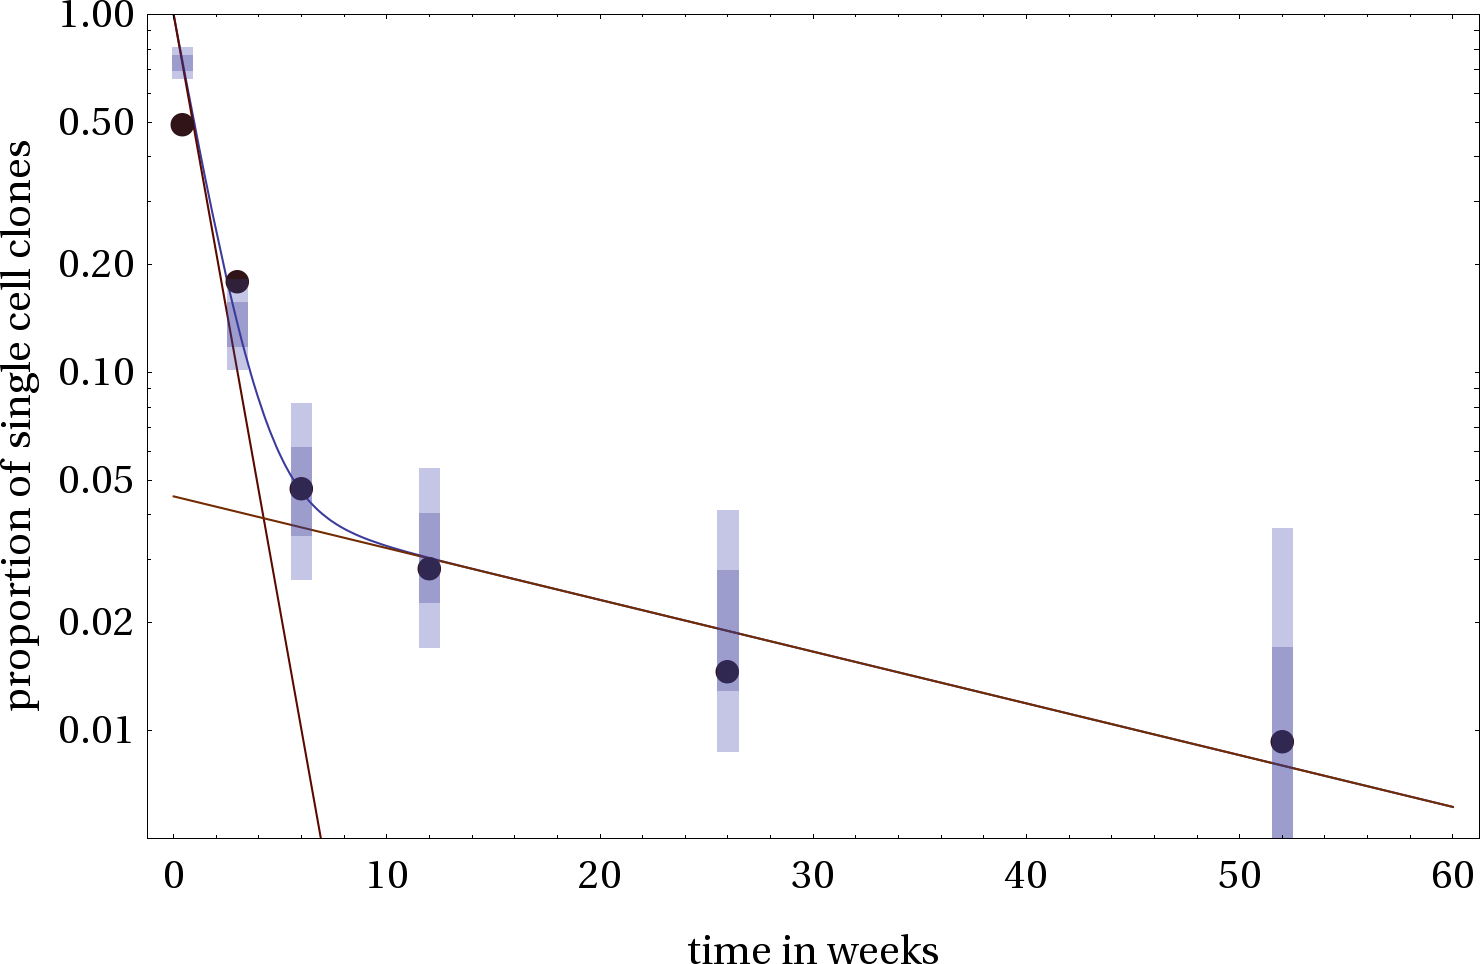
\includegraphics[height=2in]{single-cell-clones.png}\hfill~
	\caption{\label{fig:oes-stem-parameters}\textbf{Left} shows the posterior distribution for the stem cell parameters; there is a peak at $\rho_S = 0.044$, $1/\Lambda = 30~\textrm{weeks}$. \textbf{Right} shows the fit against the measured single cell clones; blue error regions are due stochastic noise, at $1$- and $2\sigma$ confidence regions; the initial steep slope is the predicted single cell frequency if there were no stem cells. }
\end{figure}

Figure \ref{fig:oes-stem-parameters} shows the results of the inference, and its fit against the observed frequencies. Obviously, with such low counts, it is hard to be very precise with the parameter fits. However, it is notable that the observed counts absolutely do not fit a model with no stem cells. The inferred division rate $\Lambda$ is reasonably free from systematic errors. On the other hand, the proportion $\rho_S$ should not be directly identified with the proportion of stem cells in the basal layer. There may be significant labelling bias, possibly even dependent on whether a given stem cell is active or not; on the other hand, it should only be a factor of a few, as opposed to orders of magnitude in error.

Given that statistically, there does indeed seem to a be population of quiescent cells, it is nature to go and look for them. Experimentally, it was suggested that the protein CD34 is a marker for stem-like behaviour. Whilst some correlations were found between single cell clones and CD34$^\textrm{High}$ cells, it was not entirely convincing. Currently, it is thought that CD34 is simply not a tight marker. Investigations are continuing.

\section{Conclusions}

We have seen how clonal size distributions which include suprabasal counts lead to a quantitative theory of epithelial maintenance. To be fashionable, one could call this full counting statistics. Using this theory we looked at three things:

\begin{enumerate}
\item Comparison of the physiologically defined proportion of proliferating cells in the basal layer with the widely accepted proliferation marker Ki67 reveals significant differences. These differences are even more pronounced in slower cycling tissues. We conjecture the existence of a stage of the cell cycle where rRNA transcription is absent.

\item We can quantitatively characterise drug effects, such as for ATRA. There, we found that the effect is an increase in division rate of progenitors, with a matching increase in stratification rates such that the overall proportion of progenitors in the basal layer remains constant.

\item Following a suggestion of functionally stem cells in the basal layer, we examined in detail the fate of single cell clones and found some circumstantial evidence in favour. Even while lacking a clear genetic marker, we were able to make some quantitative characterisation of them.
\end{enumerate}

Having this theory allows us to critically examine in great detail the accepted dogma of cell cycle, make quantitative predictions of drug effects and find evidence for further modifications to underlying cell division processes even in the face of a lack of firm biochemical signatures.

Some clear questions remain:

\begin{itemize}
\item The underlying division process used here is essentially zero-dimensional. Division and stratification occur without reference to any external feedback. In particular, homoeostasis is only maintained on average. Whilst the total number may indeed be sufficiently macroscopic that fluctuations do not matter, local density fluctuations may in fact lead to break-up of the tissue. Indeed, a combination of critical branching and local fluctuations can cause logarithmic divergence in density [??]. Investigations into models with interaction occupy the next chapter.

\item In a similar vein, as already mentioned, the scaling behaviour was crucial in overturning an incumbent stem/transit amplifying model, but became a sort of liability when inferring parameters. This is exactly the benefit of curse of universality classes. In effect, the zero-dimensional branching model is the prototypical model for a wide universality class, which all enjoy the same scaling function and growth rates. The precise underlying dynamics are hidden quite effectively. To explore those, we must probe on shorter time and length scales --- as we did for inferring the parameters. The goal, surely, is a phenomenological theory with a finite number of relevant operators, and robust experimental measurements of these; such a theory can then be relied upon by those investigating the precise biochemistry of cells.

\item The primary experimental data used so far is \emph{cohort} clonal size distributions. As such, it is not possible to perform any autocorrelation. In some ways, the lack of this information makes the pure stochastic assumption better. Nevertheless, it seems reasonable that such time lapsed data sets would be even richer in information, but it is unclear how best to exploit such information were it available.

\item The provision of homoeostasis was vital. In some ways, it is in equilibrium. True non-equilibrium processes such as development and cancer could do anything, from a purely theoretical point of view. Nevertheless, it seems a reasonable starting point to assume that such processes can be understood within the same framework, and it must be the case that the behaviour in homoeostasis constrains the ways in which it can deviate.

\end{itemize}

\chapter{\label{ch:voter}Voting on homoeostasis}

\section{Overview}

Whilst a critical Galton-Watson process (see section \ref{sec:oesophagus-scaling}) is capable of describing the clonal size distributions in, for example, oesophageal epithelium or mouse epidermis  \citep{klein07}, it is unsatisfactory for two reasons.

\begin{enumerate}
\item Homoeostasis is only maintained on average, for the entire tissue. The total number of cells in the system thus makes a one dimensional random walk, with an absorbing boundary which can be ignored in the macroscopic limit; self-consistently we may take the continuum (Fokker-Planck) limit and obtain a simple diffusion, spreading with time with width $~\sqrt{t}$. However, whilst the total number may be macroscopic, the local density is not; the observation of maintained uniform density in oesophageal epithelium motivates a theory of spatial densities, with interactions.

\item The oesophageal epithelium is intrinsically two dimensional; other tissues maybe three dimensional, or even one dimensional (e.g. intestinal crypts). The study of equilibrium universality classes alerts us to the possibility of exceedingly rich structure in low dimensions, motivating a similar expectation for non-equilibrium processes. In addition, the clonal data naturally available comes with two dimensional structure --- each clone may be trivially imaged. The spatial correlations no doubt provide extra constraints on the underlying microscopic model.

\end{enumerate}

The simplest extension of the one-type Galton-Watson process considered in section \ref{sec:oesophagus-scaling} is the \emph{voter model} \citep[][chapter V]{liggettbook}. The basic intuition is a network of voters (cells) who randomly change their opinion (genetic label) to match one of their neighbours. This may generically happen on any graph, but we are mostly concerned with some approximation to $d$-dimensional spaces. This is a well studied model, and we proceed to review the existing work on this, and make some conjectures based on Monte-Carlo simulations. The primary conjecture will be that, at least in 2D (and thus above), it is the prototypic system of a wide universality class, including multi-type division processes and cellular migration \citep{klein08}. As such, we are interested in its universal and leading order perturbations.

The existing literature broadly falls into two approaches, separated by a language barrier. On the one hand, there is a mathematical literature which details exact results about the classic voter model on square $d$-dimensional lattices; results are rigorous but limited. On the other hand, there is a phenomenological approach which has its roots in the study of critical dynamics, through the use of Langevin equations and renormalisation group as applied to non-equilibrium systems; the results are then of course non-rigorous but explore more of the theory space. The two approaches thus complement each other, and taken together gives good intuition about the voter model and its generalisations.

\section{Exact results}

The classical voter model \citep{voter1,voter2} is defined to be a Markov process $\eta_t(x)$ with $x \in \mathbf S$, $\eta_t \in \mathbf X=\{-1,1\}^\mathbf{S}$, where $\mathbf S$ is some set of positions. The rates of opinion changes are:
\begin{equation*}
c(x, \eta) = \begin{cases}
\sum_y p(x,y) \delta_{\eta(y),1} & \textrm{if $\eta(x) = -1$}, \\
\sum_y p(x,y) \delta_{\eta(y,-1} & \textrm{if $\eta(x) = 1$},
\end{cases}
\end{equation*}
where $p(x,y) \ge 0$ for $x,y \in \mathbf{S}$ and $$\sum_y p(x,y) = 1 \qquad \textrm{for $x \in \mathbf{S}$}.$$ In other words, a voter at $x$ waits for a unit time and then chooses to flip to match another site $y$ which is chosen with probability $p(x,y)$.

We shall be mostly dealing with $\mathbf S = \mathbb{Z}^d$, square lattices in $d$ dimensions, and possibly $\mathbf S = \mathbb{T}_N^d$, $d$-dimensional tori with sides $N$ (when we wish to examine finite size effects); interactions are also taken to be nearest-neighbour only, i.e.\ $p(x,y) = 1/2d$ for $\left| x - y \right| = 1$. Some of the results quoted in this chapter will be true for less restrictive conditions.

\citet{liggettbook} shows that on $\mathbb{Z}^d$, for $d \le 2$ the only stationary states are $\eta(x) = -1\textrm{ or }1, \forall x$, and for $d \ge 3$ there is a family of stationary states, with parametrised by the proportion of positive voters $\theta$, which are translation invariant. Thus in two dimensions and below, the system orders and above it does not.  However, it is the case that in all dimensions, if we start with an initially disordered state then $\eta_t(0)$ changes state infinitely often as $t \rightarrow \infty$; thus even in low dimensions the system avoids being trapped. We may also approach the question of ordering by considering the density of interfaces, i.e.\ neighbours with opposing opinions. Then it is found that in $d=1$ the density $\rho_t \sim 1/\sqrt{t}$ whilst in $d=2$, $\rho_t \sim 1/\log t$. 

On a torus $\mathbb{T}_N^d$ of side $N$, due to the finiteness, the system will always order, with finite time. \citet{voterconsensus} considers the consensus time of an initially disordered state: $$\tau^{(N)} = \inf \left\{ t \ge 0 : \eta_t(x) = \textrm{$-1$ or $1$}, \forall x \in \mathbb{T}_N^d \right\}.$$ As functions of $N$, the average consensus time diverges as:
\begin{equation*}
E\left[\tau^{(N)}\right] = -\left[\theta \log \theta + (1-\theta) \log (1-\theta) \right]\times\begin{cases}
\frac{1}{6} N^2           & d = 1 \\
\frac{2}{\pi} N^2 \log N  & d = 2 \\
K~N^d                     & d \ge 3
\end{cases}
\end{equation*}
where $\theta$ is the initial density of positive votels, and $K$ is an unhelpful constant. \citet{voterconsensus} also finds the exact distribution of consensus times, but they do not have simple forms.

Especially relevant for clonal counting is the behaviour of an initially single positive voter. \citet{bramson&griffeath} studied this case for $\mathbf{S} = \mathbb{Z}^d$. They find that the average size $N_t = \left| \left\{x: \eta_t(x) = 1\right\} \right|$, conditioned on $N_t > 0$ grows asypmtotically:
\begin{equation*}
E\left[N_t\middle|N_t>0\right] \overset{t \rightarrow \infty}{\longrightarrow} \begin{cases}
\sqrt{\pi\,t}         & d = 1 \\
\frac{\pi\,t}{\log t} & d = 2 \\
\gamma_d\,t           & d \ge 3
\end{cases}
\end{equation*}
where $\gamma_d$ is the probability that the simple random walk never returns to its initial position. Furthermore, they find the limiting distributions
\begin{equation*}
\lim_{t\rightarrow\infty} P\left[\frac{N_t}{E\left[N_t\middle|N_t>0\right]} \le u \middle| N_t > 0\right] = \begin{cases}
1 - e^{-\pi\,u^2/4} & d = 1 \\
1 - e^{-u}     & d \ge 2
\end{cases}
\end{equation*} for $u \ge 0$. However, as we shall see below, for $d=2$ the convergence is extremely slow, and so for practical time scales the limiting distribution never occurs.

\paragraph{Coalescing random walk}

Much of the work referenced above exploits a duality of the voter model with a system of coalescing random walkers. Specifically, the probability of of the voter model starting in state $\eta_0$ and ending at $\eta_t$ is the same as starting a system of walkers in state $\eta_t$ and evolving backwards in time to $\eta_0$, a time $t$ later. This is easiest seen graphically (figure \ref{fig:voter-model-duality}).

\begin{figure}[htb]
	\centering
	\includegraphics[width=2.2in]{voter-model-duality.png}
	\caption{\label{fig:voter-model-duality}Duality between voter model and coalescing random walk. Notice that for a given history $\eta_t$ the duality only applies for the start and end states, and not the states in the middle.}
\end{figure}

Note that nothing is said about intermediate states --- no equivalences exist there --- the duality applies only to the initial and final states. As an example of its use, consider trying to find the size of the patch containing the origin in a multi-type voter (each voter has more than two opinions). The origin and another location $y$ will have the same opinion iff there the walkers starting there meet at some time $\tau < t$; this is equivalent to asking if a single random walk starting at the origin will reach $y$ within time $2t$, the result of which is known from the seminal works of Erd\"os.

\section{Generalised voter universality class}

The Landau theory of equilibrium phase transitions works phenomenologically, by including in the action all terms allowed by the symmetries of the problem. This is then supplemented by renormalisation group theory, which assures us that under coarse-graining these terms will approach a fixed point. We then identify these fixed points as different phases or phase transitions, and classify them by the number of relevant directions they have in parameter space, i.e.\ the number of potential perturbations which would cause the renormalisation flow to diverge.

In principle, there is nothing in this prescription which requires an equilibrium statistical system. At least formally, any system for which we may write a partition function and can perform the necessary expansions are susceptible. In practice of course, we are extremely limited. Nevertheless, the class of classical non-equilibrium phenomenon has been well studied, and that includes the voter model. Indeed, it actually includes considerable generalisations to the voter model. The class we will consider below are defined by, as always, its dimensions and symmetries: we consider an order parameter which is a single component field $\phi$ representing the local ``magnetisation'' --- e.g.\ $+1$ is labelled, $-1$ is not; we require the theory to be symmetric under $\phi \rightarrow -\phi$; and there be no fluctuations when $\phi=\pm 1$, i.e. they are absorbing states. This class we shall denote the \emph{generalised voter model}.

At this point, it is worth building some intuition by translating the results of the previous section into more ``physicist'' language. The lack of stationary states in one and two dimensions, apart from the trivial absorbing ones, is a sign of macroscopic ordering --- the order parameter breaks the $\mathbb{Z}_2$ symmetry. In three dimensions, such ordering is not guaranteed --- indeed, it can be shown that it is almost certain the overall magnetisation will not change from the initial starting value. In fact, $d=2$ is a critical point --- it is known that random walk recurrence is critical there, and we can see evidence for it in the various logarithms which appear in the asymptotic results as a result of critical slow down. However, the fact that it is logarithmic and not some power law implies a potential failure of naive perturbation theory, something which we shall need to be careful about.

\subsection{Directed percolation}

The theory of single component, \emph{single} absorbing state is that of \emph{directed percolation} \citep[][section 10.6]{cardybook}. Because this is a well-studied system, we use it as a road-map for a similar attempt at the generalised voter model.

Let $\phi(r,t)$ describe the local density of a population. Extremely relevant for us is the fact that $\phi(r,t) >= 0$, and $\phi(r,t)=0~\forall r,t$ is an absorbing state --- no fluctuation can restore an extinct population. We thus postulate a Langevin equation to describe the dynamics of this variable: 
\begin{equation}
\partial_t \phi = D \nabla^2 \phi + \lambda \phi - \mu \phi^2 + \zeta + \ldots, \label{eq:DP-langevin}
\end{equation}
where $\zeta$ is a noise term, generated by self-interaction. We have neglected higher terms in $\phi$ and its derivatives, because they will turn out to be irrelevant near the upper critical dimension ($d=4$). The constants $\lambda$ and $\mu$ may be understood as a birthday and death rate due to over-crowding. In the absence of diffusion and noise there would a dynamic phase transition at $\lambda=0$; for $\lambda < 0$ the population always eventually dies out whilst for $\lambda > 0$ there exists a steady state with $\phi = \lambda/\mu$.

\newcommand{\tphi}{\ensuremath{\tilde \phi}}
\newcommand{\tJ}{\ensuremath{\tilde J}}

The noise term $\zeta$ is constrained to vanish whenever $\phi$ does. Thus we may consider an approximation $$\zeta = F_0(\phi) + \mu^\prime \phi \eta + \ldots$$ where $F_0(\phi)$ is some function of $\phi$ and its derivatives, and thus may be absorbed into the definitions of $D$, $\lambda$, $\mu$, etc.\ and will henceforth be ignored, $\eta$ is a Gaussian noise source of zero mean and unit variance with no temporal spatial correlations, and neglected terms will again turn out to be irrelevant. 

Physical quantities may be considered as averaging over values of $\phi$ and $\eta$ which obey equation \eqref{eq:DP-langevin}:
\begin{align*}
Z &= \int \mathcal{D}\phi \mathcal{D}\eta~\delta\left(-\dot \phi D \nabla^2 \phi + \lambda \phi - \mu \phi^2 + \mu^\prime \phi \eta \right) e^{-\eta^2/2} \\
&= \int \mathcal{D}\phi \mathcal{D}\tphi \mathcal{D}\eta~\exp\left\{-\int_{r,t}~\left[\tphi \left(-\dot \phi + D \nabla^2 \phi + \lambda \phi - \mu \phi^2 + \mu^\prime \phi \eta \right) + \frac{\eta^2}{2} \right] \right\} \\
&= \int \mathcal{D}\phi \mathcal{D}\tphi~\exp\left\{-\int_{r,t}~\left[\tphi\dot{\phi} + D \nabla \tphi \cdot \nabla \phi - \lambda\tphi\phi + \tphi\phi\left(\mu\phi - \mu^\prime\tphi \right) \right] \right\} 
\end{align*}
where we introduce the \emph{response field} $\tphi$ and integrate over the Gaussian noise $\eta$ which only appears quadratically. The resulting action functional, with the usual fictitious linear source terms
\begin{equation}
S[J,\tJ] = \int_{r,t}~\left[\tphi\dot{\phi} + D \nabla \tphi \cdot \nabla \phi - \lambda\tphi\phi + \tphi\phi\left(\mu\phi - \mu^\prime\tphi \right) - J\phi - \tJ\tphi \right]
\end{equation}
may then be analysed with the usual field theoretic methods, to yield critical exponents. In particular, a powerful numerical method based around \emph{non-perturbative renormalisation group} \citep{DPnprg} is capable of handling potentially troublesome anomalous scaling of coherence length, such as the Kosterlitz--Thouless transition, without putting in non-perturbative elements such as vortices by hand.

\subsection{Voter model}

\citet{voterlangevin} proposed, for the generalised voter model:
\begin{equation}
\partial_t \phi = D \nabla^2 \phi + (a \phi - b \phi^3)(1-\phi^2) + \sigma \sqrt{1-\phi^2} \eta, \label{eq:voter-langevin}
\end{equation}
where again $\eta$ is a Gaussian noise source with zero mean and unit variance. Although equation \eqref{eq:voter-langevin} is motivated by the possibility of multiple transitions, it is also thought to be complete with respect to the relevant terms.

\citet{canet05} then undertakes a non-perturbative renormalisation group analysis of equation \eqref{eq:voter-langevin}; in one dimension they find a critical point corresponding to the critical voter dynamics, and a stable point corresponding to an annihilating random walk; in two dimensions they find that the only stable fixed point is the voter model; in three dimensions and above, only the Gaussian point --- disordered state --- is stable.
 
\section{Monte-Carlo simulations}

\citet{dornic01} has considered a variety of modifications of the voter model, and concludes that it is the basin of attraction of a wide range of models; this is obviously supported by the renormalisation group analysis by \citet{canet05}.

Broadly however, the interest has not been concentrated on clone size distributions. Although the theoretical work of \citet{bramson&griffeath} gives the limiting distributions, it does not give indications of the rates of convergence; in particular, in two dimensions (i.e.\ critical) the convergence appears to be very slow (figure \ref{fig:voter-clone-size-distribution}). Thus we performed some Monte-Carlo simulations of the voter model, starting with one single labelled cell, and observing the size distribution of surviving clones. For computational efficiency we actually simulate a multi-type voter distribution where each initial cell is labelled with a different colour; this also allows easy visualisation of the coarsening process (figure \ref{fig:multitype-voter-coarsen}).

\begin{figure}[htb]
	\centering
	\hfill
\includegraphics[width=128pt]{voter-coarsen/1.png}
	\hfill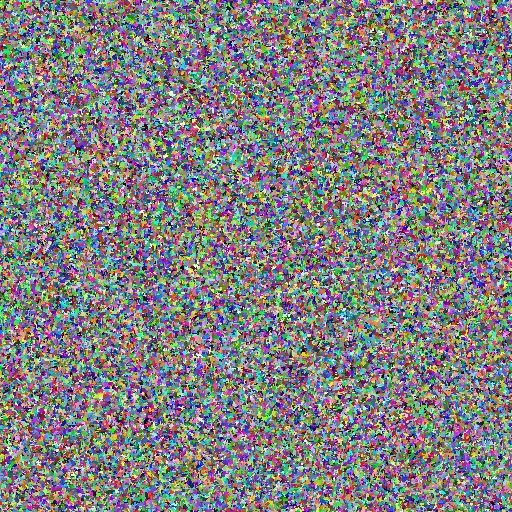
\includegraphics[width=128pt]{voter-coarsen/4.png}
	\hfill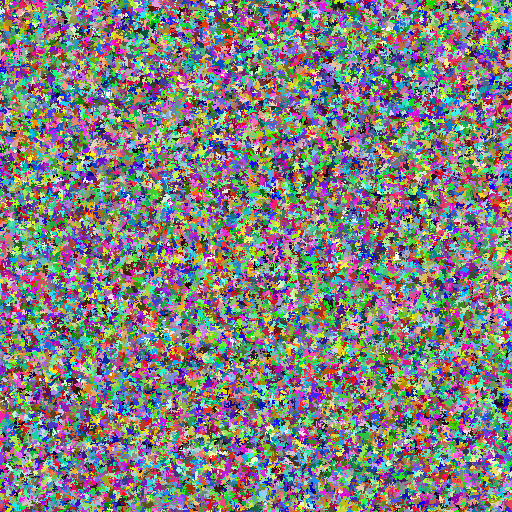
\includegraphics[width=128pt]{voter-coarsen/16.png}\hfill~\\
	\vspace{0.1in}
	\hfill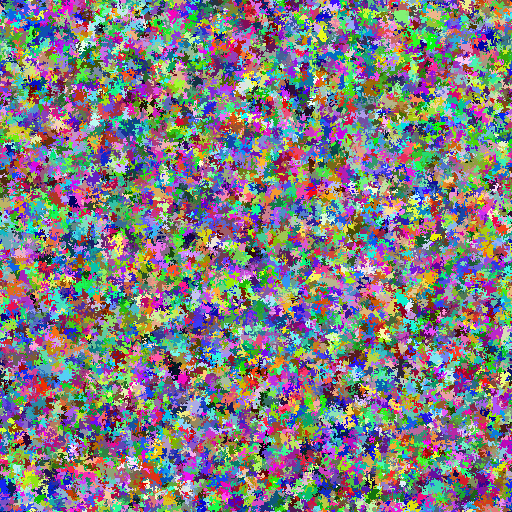
\includegraphics[width=128pt]{voter-coarsen/64.png}
	\hfill\includegraphics[width=2in]{voter-coarsen/256.png}
	\hfill\includegraphics[width=2in]{voter-coarsen/1024.png}\hfill~\\
	\caption{\label{fig:multitype-voter-coarsen}The classic voter model shows coarsening with length scale proportional to $\log(t)$; shown are typical multi-type voter process at times $t=1,4,16,64$, in units of mean voter opinion change. }
\end{figure}

\begin{figure}[htb]
	\centering
	%\includegraphics[width=2.2in]{}
	\caption{\label{fig:voter-clone-size-distribution}Clone size distribution (cumulative) of the classic voter dynamics in two dimensions. The limiting distribution for is exponential \citep{bramson&griffeath}, but the approach is extremely slow. For all practical times, there is a small reduction in small clones and a ``hump'' which moves left.}
\end{figure}

It is also possible to insert post-mitotic cells into the simulation, and obtain a system similar to \citet{klein08}. Here however, we are interested in clonal distribution as opposed to clustering of progenitor cells. In particular, we can modify the amount of diffusion of vacancies left by stratified post-mitotic cells; this essentially introduces long-ranged interactions into the model. Preliminary observations indicate that the model becomes quite sensitive to initial conditions. In particular, it is possible to get a clone size distribution which really is exponential; alternatively, it is possible to get one which has an excess of small clones, rather than the usual reduction.

\section{Conclusions}

As \citet{dornic01} points out, a crucial feature of the voter model is a lack of surface tension. Labelling experiments introduce boundaries which are physiologically meaningless, and must therefore be devoid of surface tension. Further, (genetic) labelling clearly has two absorbing states, and the dynamics is symmetric under exchange of labelled and non-labelled cells. As we have seen, there is considerable evidence that the critical dynamics falls into the universality class of a generalised voter model.

Our Monte-Carlo simulations have the following interpretation: there are two length scales in the problem --- the coherence length, i.e.\ typical clone size, and the interaction length, which is roughly how far a replacement cell is from the stratified one. At early times in a labelling experiment, the coherence length is short, and potentially shorter than the interaction length; in this regime, the dynamics is essentially mean-field and a rapid convergence to exponential scaling occurs; once the coherence length increases sufficiently, any deviations from the limiting exponential distribution only decays slowly, possibility logarithmically. If instead some other non-representational labelling occurs, then a different deviation from scaling will be frozen in. This ability to freeze in the microscopic dynamics is surely useful.

Some potential directions are:

\begin{enumerate}

\item Obtain the leading order corrections to the exponential scaling function, or at least conjecture one.

\item Extend the work of \citet{canet05} using the non-perturbative renormalisation group to understand the leading irrelevant operators (since there does not appear to be any relevant ones).

\item Link the phenomenlogical parameters in equation \eqref{eq:voter-langevin} to a microscopic theory. In conjunction with understanding of irrelevant operators, this would allow inference of microscopic parameters.

\item Break the assumption of homoeostasis, but maintain the spatial interactions. It is observed sometimes that signalling boundaries during development are not sharp, but become so over time. Could this be fully accounted for by a theory of interacting progenitors which are not in homoeostasis?

\end{enumerate}

\chapter{\label{ch:spinal-chord}Spinal chord}

\paragraph{Overview}

This work is in a very preliminary stage, as such the focus is on understanding anatomy and fixing an overall framework within which further work can be developed. The tissue under scrutiny here is the development of spinal chord in chick; however, since the spinal chord is a highly conserved feature across many members of \emph{chordata}, we expect the conclusions to be widely applicable. The work herein is done is collaboration with James Briscoe and Anna Kicheva at MRC NIMR in Mill Hill, London.

\paragraph{Anatomy}

Spinal cord forms a pseudo-stratified tissue in which cells are organised in domains which lie parallel along the anterior-posterior (AP) axis. The width of the domains along the dorsal-ventral (DV) axis changes through development, as does the thickness along the apical-basal (AB) axis. The cells move to the apical surface during mitosis, and then move back. Fully differentiated neurons migrate out of the pseudo-stratified layer. Note that there is no clear physiologically defined boundary between the progenitor domains and the mature neurons, e.g. such as the stratified layers in epidermis/oesophagus or a separating membrane. Although there is a slight morphological difference in that progenitors are elongated and post-mitotic cells are more round, having detached from the apical end, the main differentiator is the progenitor marker Sox2; there is also the mature neuron marker p27, but its build up is delayed with respect to the down regulation of Sox2, and so can under-report; as such, we use Sox2 as ground truth.

\begin{figure}[h]
	\begin{center}
		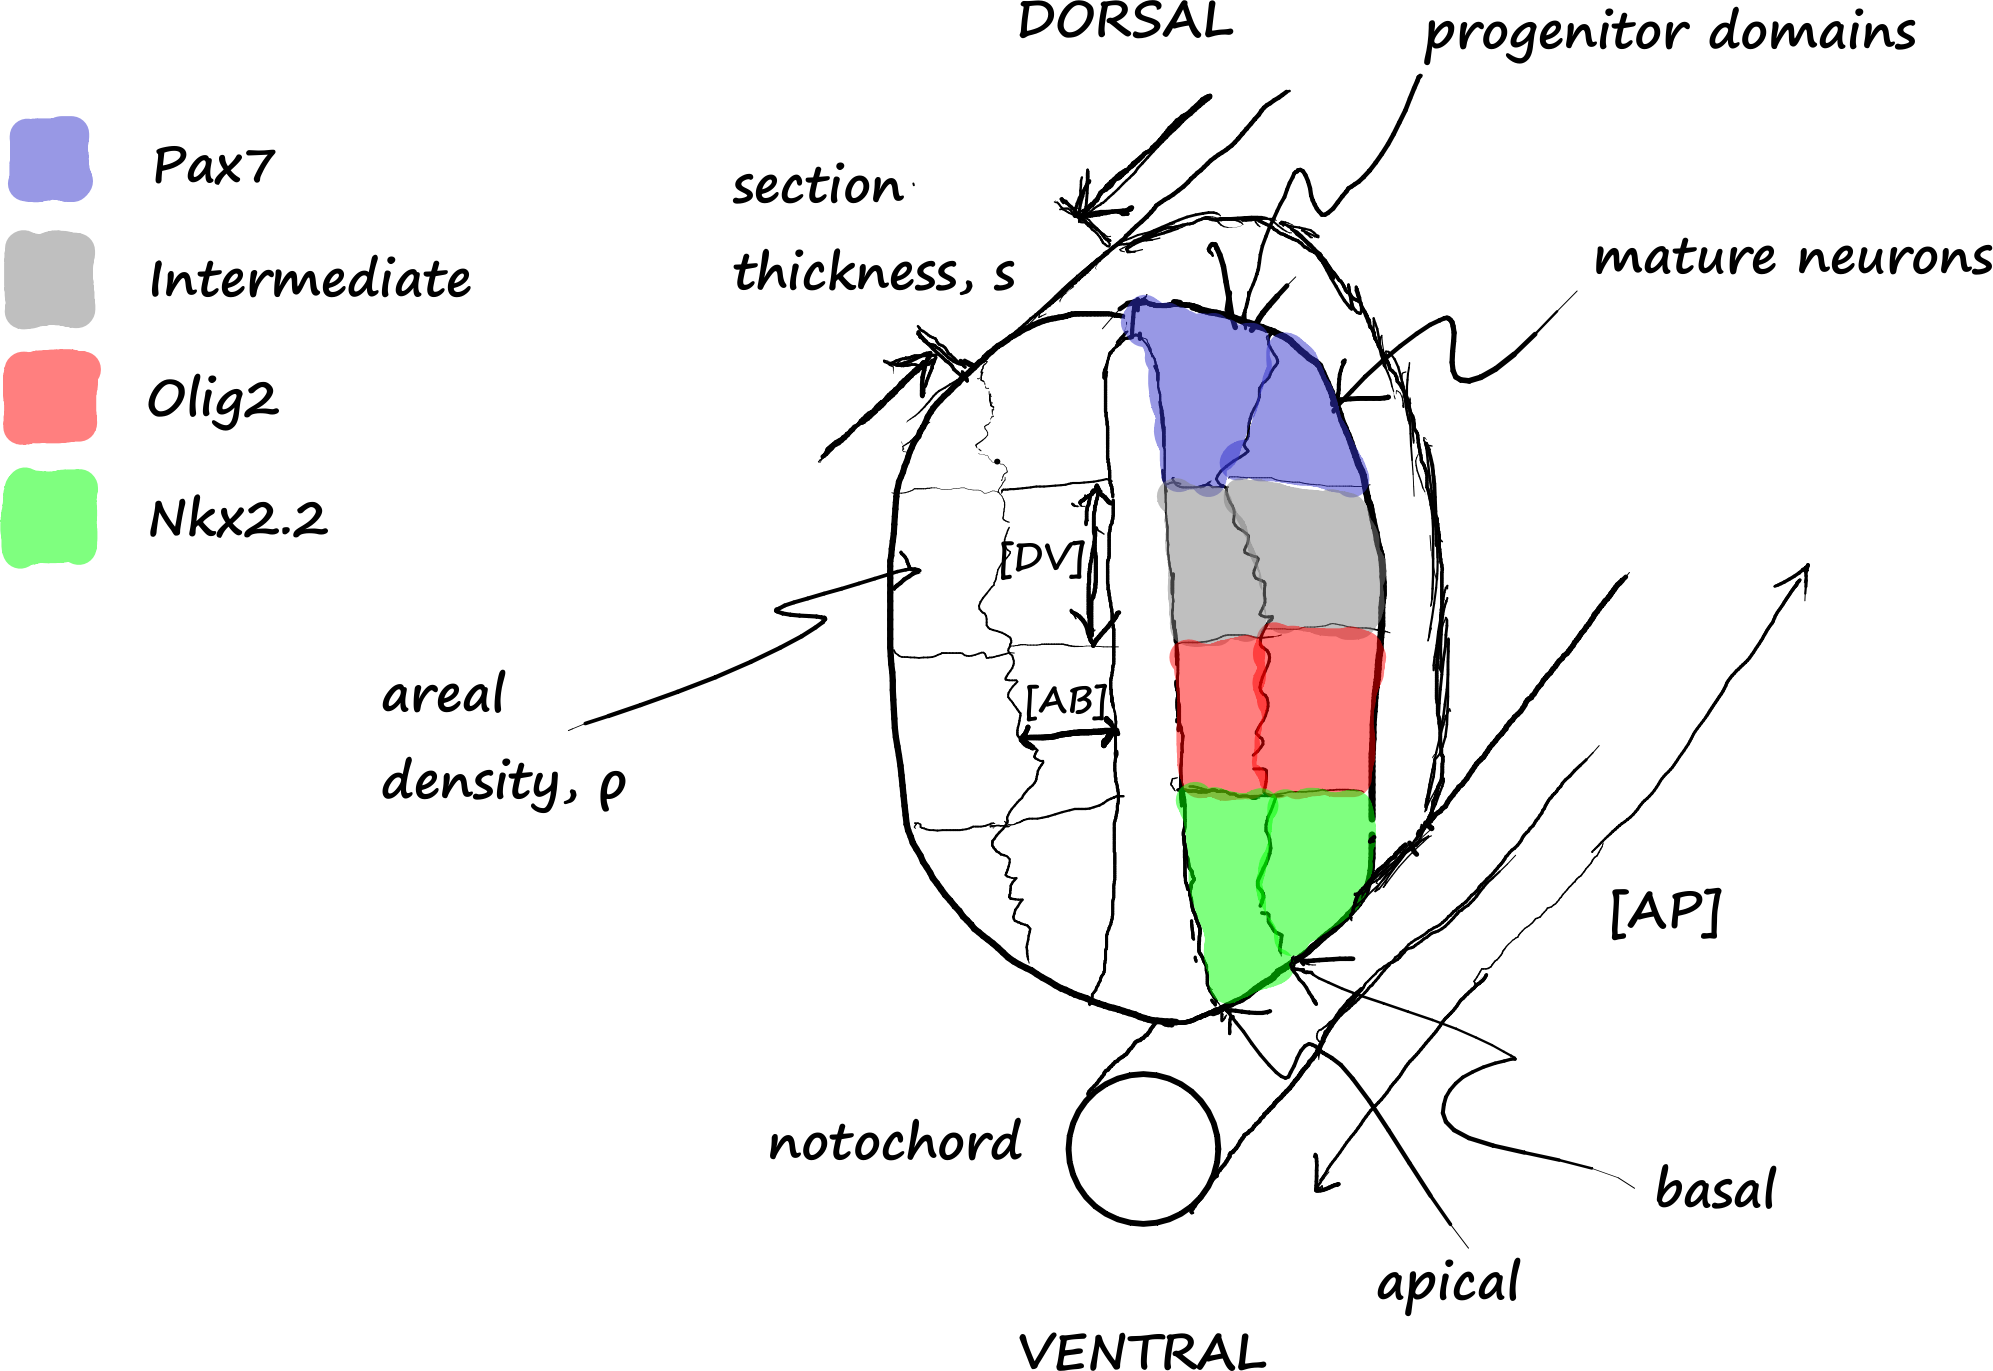
\includegraphics[width=3in]{spinal-chord-anatomy.png}
	\end{center}
	%\label{fig:anatomy}
\end{figure}

\paragraph{Division process}

In 24 hour EdU incorporation studies, it is observed that the entire progenitor domain is EdU+, as well as some mature neurons. From the number of neurons produced which are EdU- we can infer the number of post-mitotic cells in the progenitor domains at the start of the 24 hour period. A rough count of a Pax7 domain showed that around 30 mature neurons are produced during this period, of which 10 are EdU-; there are around 200 progenitors in the domain to begin with, thus only around $5\%$ of the cells are post-mitotic. However, it is observed that $100\%$ of cells in the progenitor domains express Sox2, implying that it has a moderate decay period. Further, it is observed (based only on two observations) that post-mitosis migration takes around 7 hours, with very little variance; it is also thought that division rates are around 20--30 hours. This is sufficiently long that for accurate statistics, the time spent migrating should not be ignored.

As such, the following model is proposed:

\begin{figure}[h]
	\begin{center}
		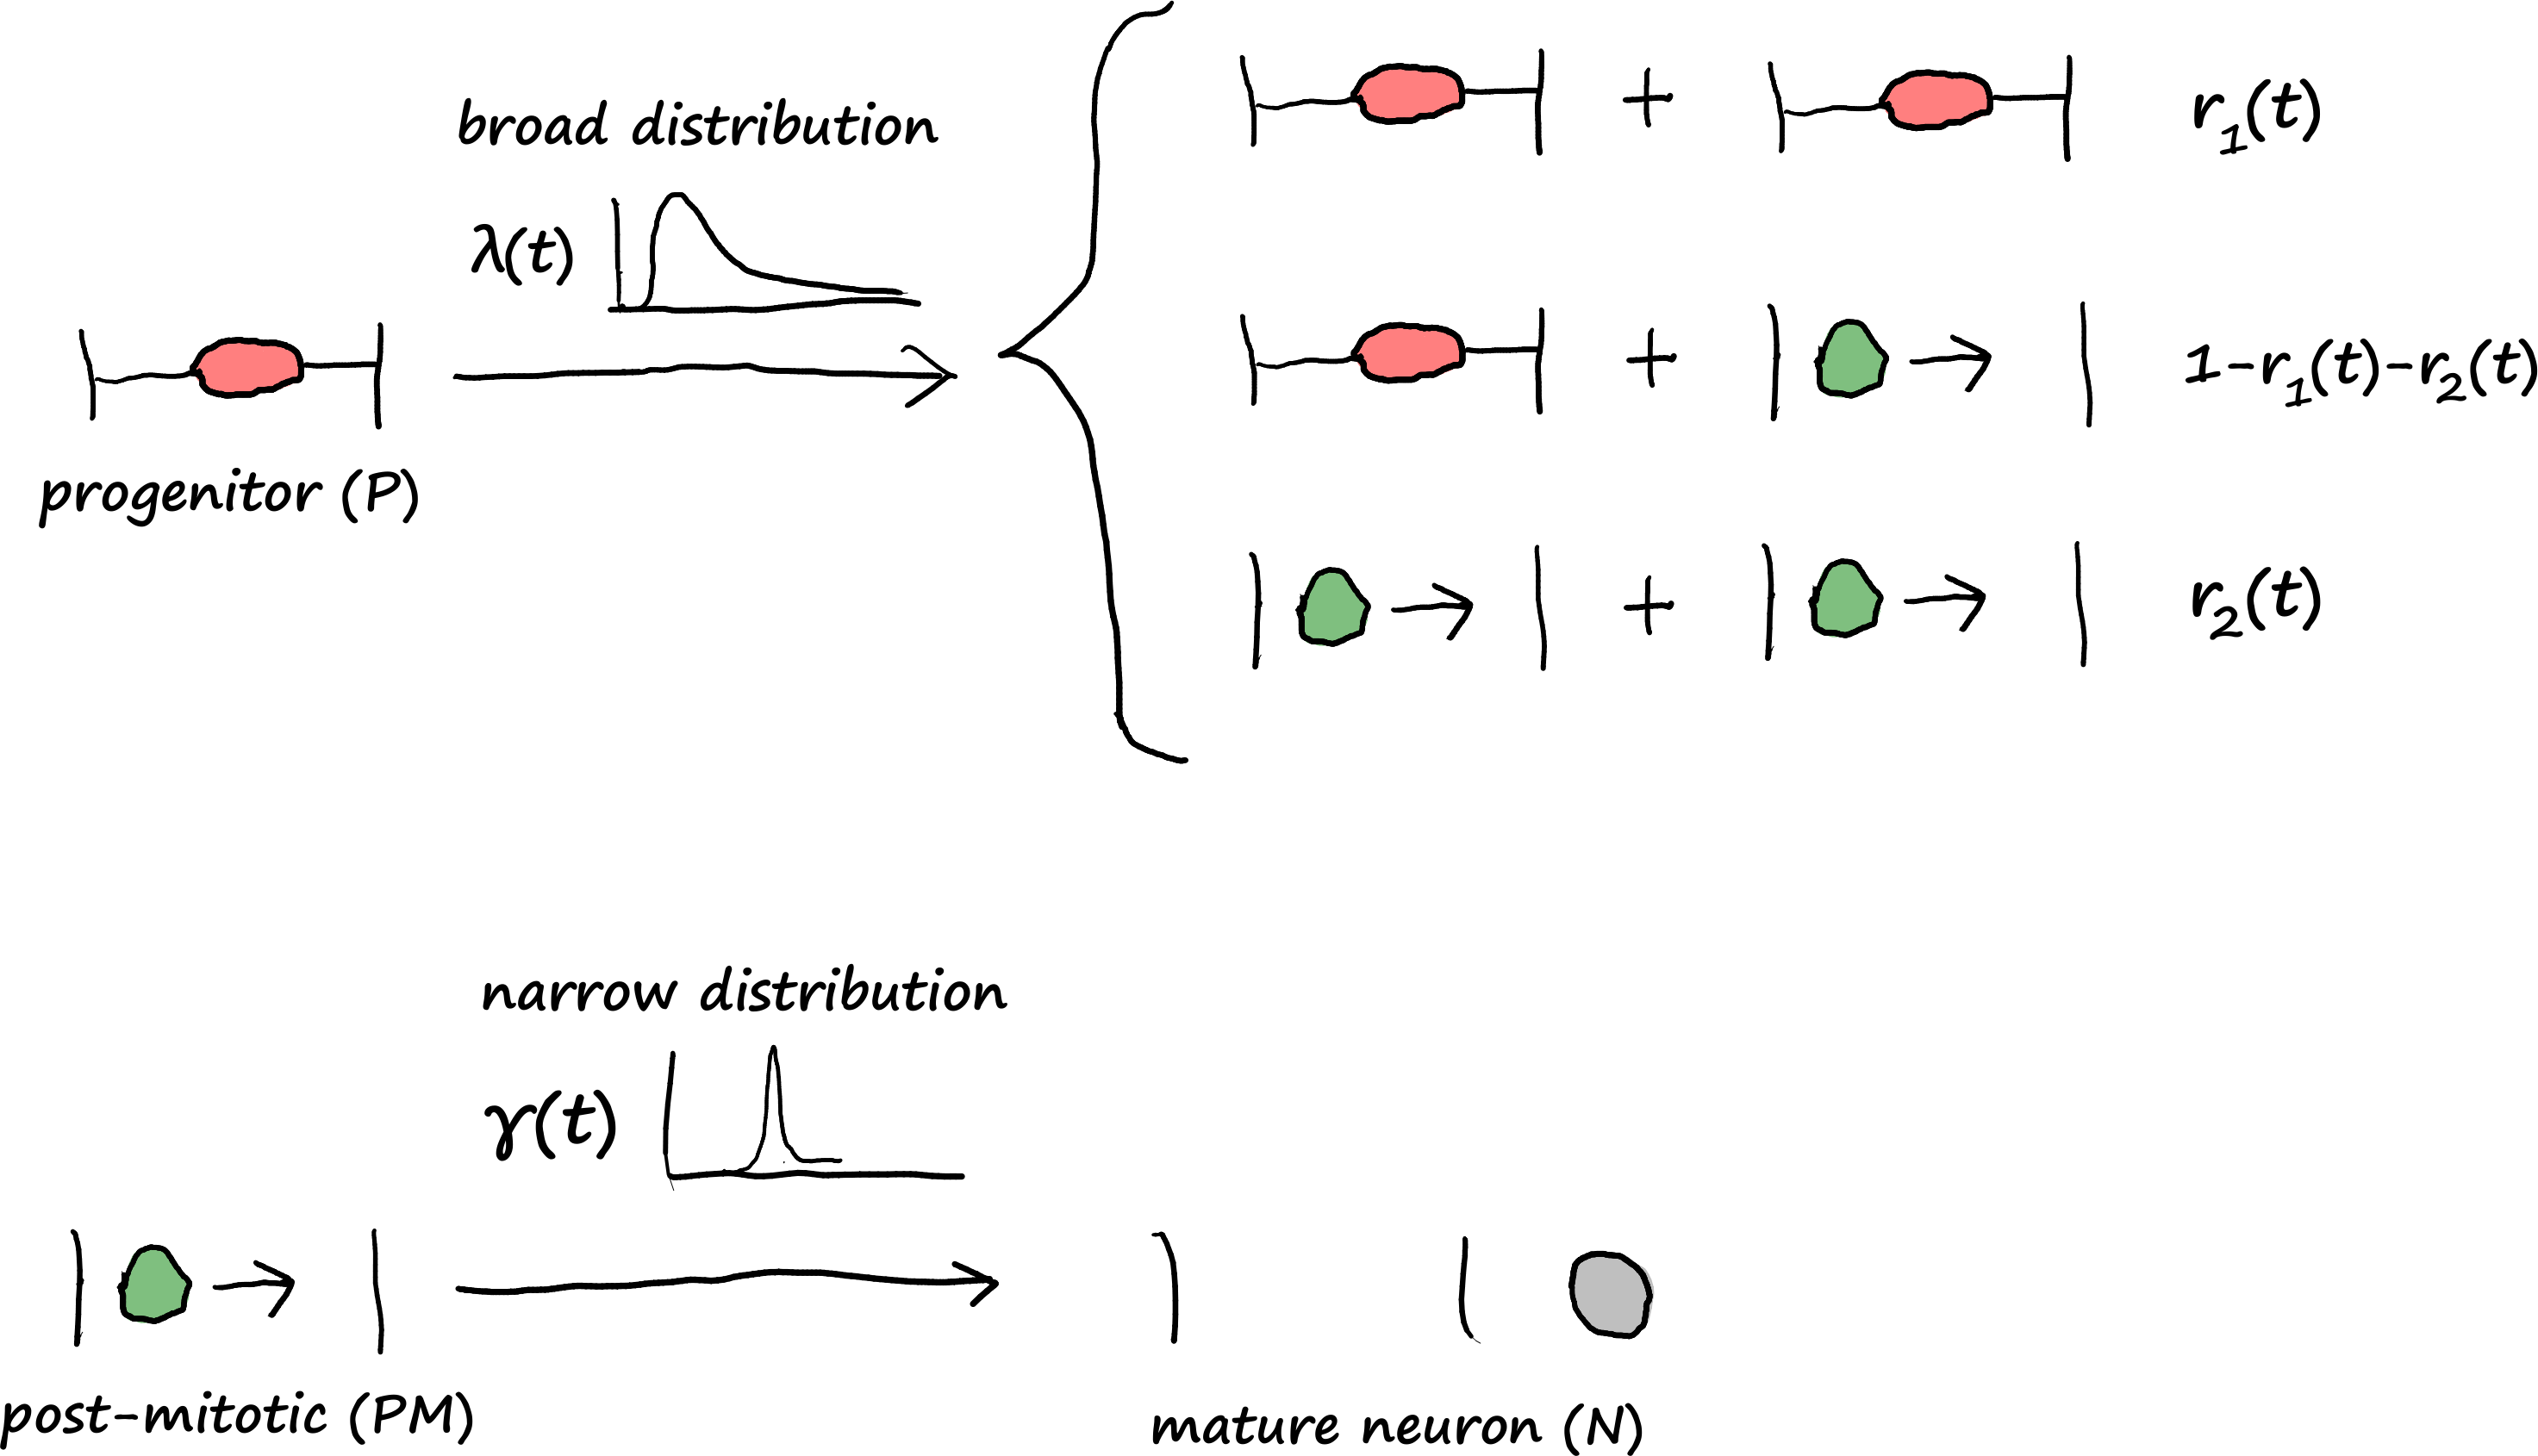
\includegraphics[width=4.4in]{division-process-A.png}
	\end{center}
	%\label{fig:division-process-A}
\end{figure}

For a first stab at modelling, it is probably sufficient to treat $\lambda(t)$ as exponential, i.e.\ perfectly stochastic, and $\gamma(t)$ as a $\delta$-distribution, i.e.\ perfectly synchronous.

Notice that if it is the case that the daughters of a progenitor independently make a decision about differentiation, then we expect the relation: $\sqrt{r_2 (t)} = 1 - \sqrt{r_1(t)}$.

\paragraph{Preliminary results}

At the moment, we have access to various data relating to sections in the transverse (AB/DV) plane, which are around $s = \SI{6}{\micro\metre}$ in thickness. From these sections, it is possible to measure the \textbf{cell density per unit area} $1/a_d$ in the progenitor domains, and the \textbf{number of progenitors and neurons}, $p_d$ and $n_d$, respectively. The domains are also roughly rectangular, and to a certain extent we can assign some \textbf{absolute dimensions} $[DV]_d$ and $[AB]_d$; however, the actual area of the progenitor domains are more accurately measured by $p a$, as opposed to $[DV][AB]$. The absolute dimensions will have more direct impact on signalling.

\begin{figure}[h]
	\begin{center}
		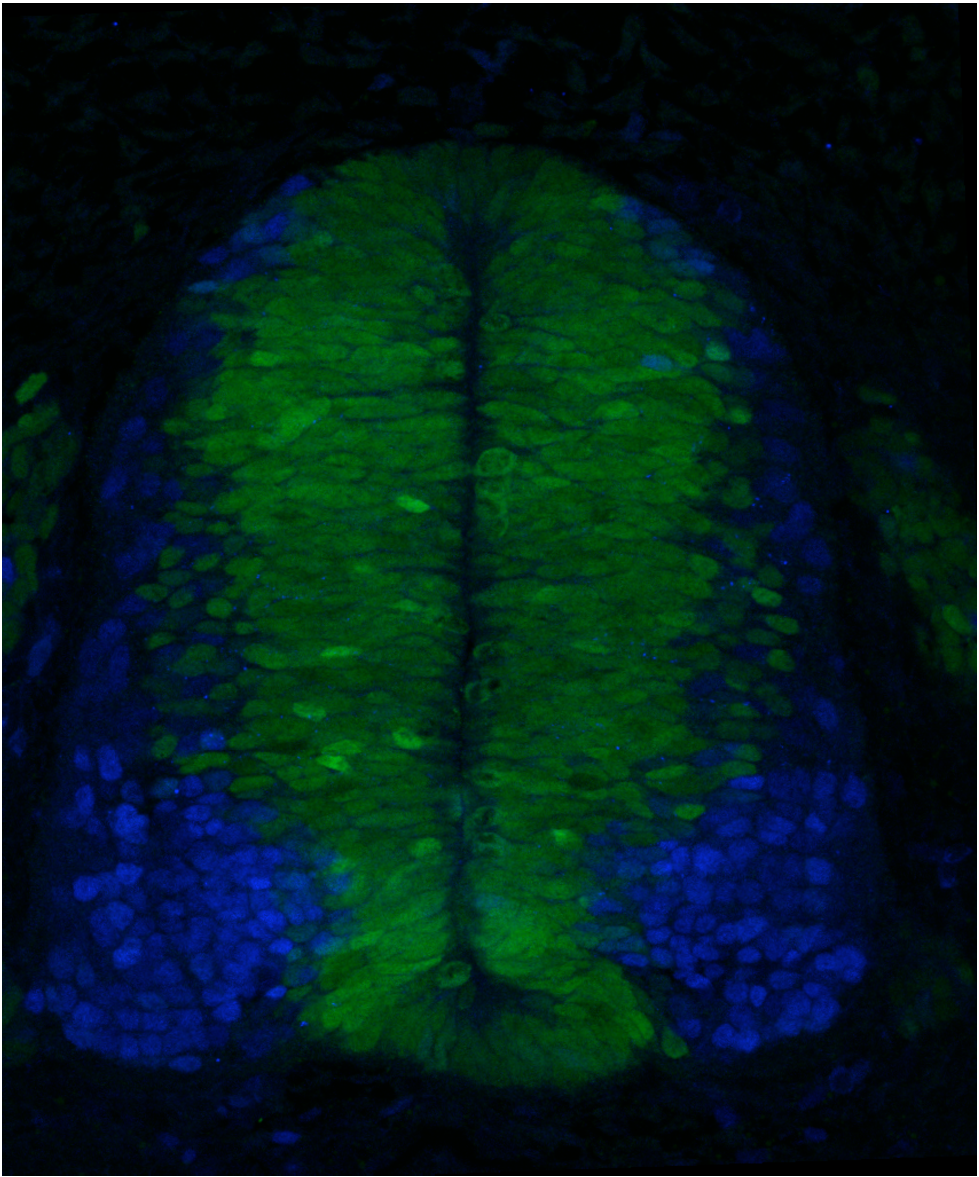
\includegraphics[height=3in]{transverse-stained-sox2-p27.pdf}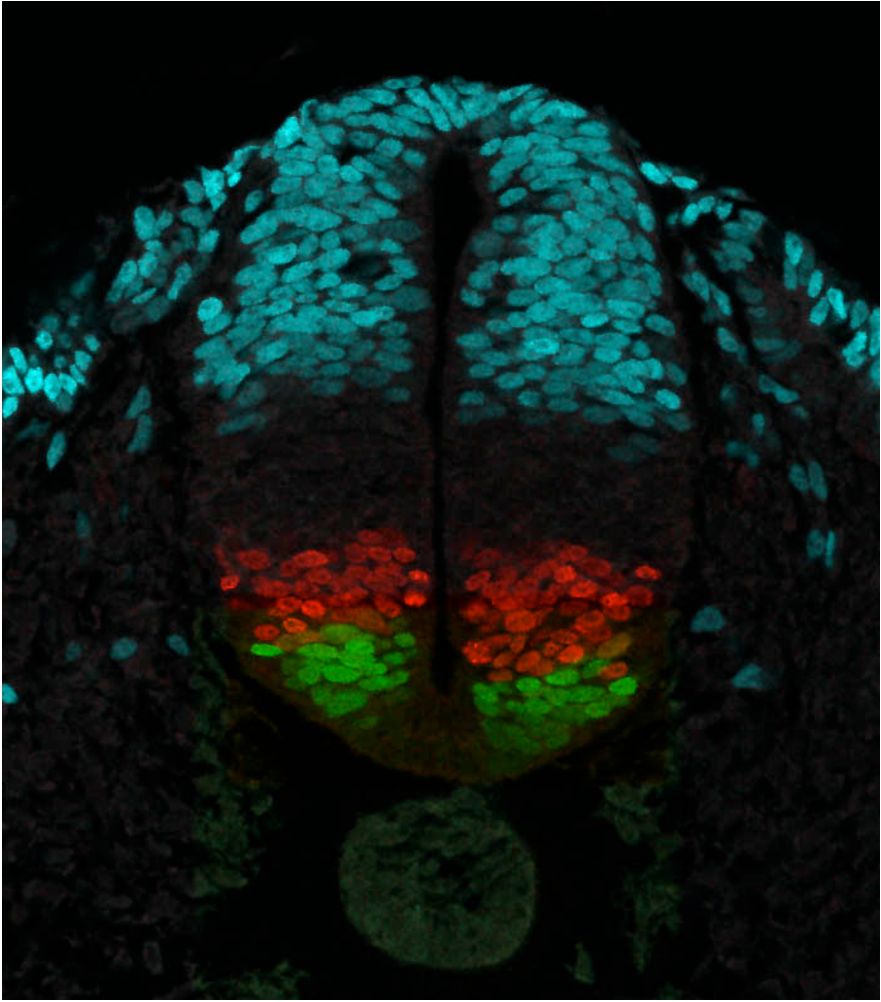
\includegraphics[height=3in]{transverse-stained-domains.pdf}
	\end{center}
	%\label{fig:stained-samples}
\end{figure}

We made/are in process of making consistency checks to the effect that these two areas should not diverge too dramatically. We calculate the \textbf{cell depth} $b$ (as measured in the AP direction) by $$b_d = \frac{[AB]_d[DV]_d s_d}{p_d a_d}.$$ We should see a reasonably tight distribution:

\begin{figure}[h]
	\begin{center}
		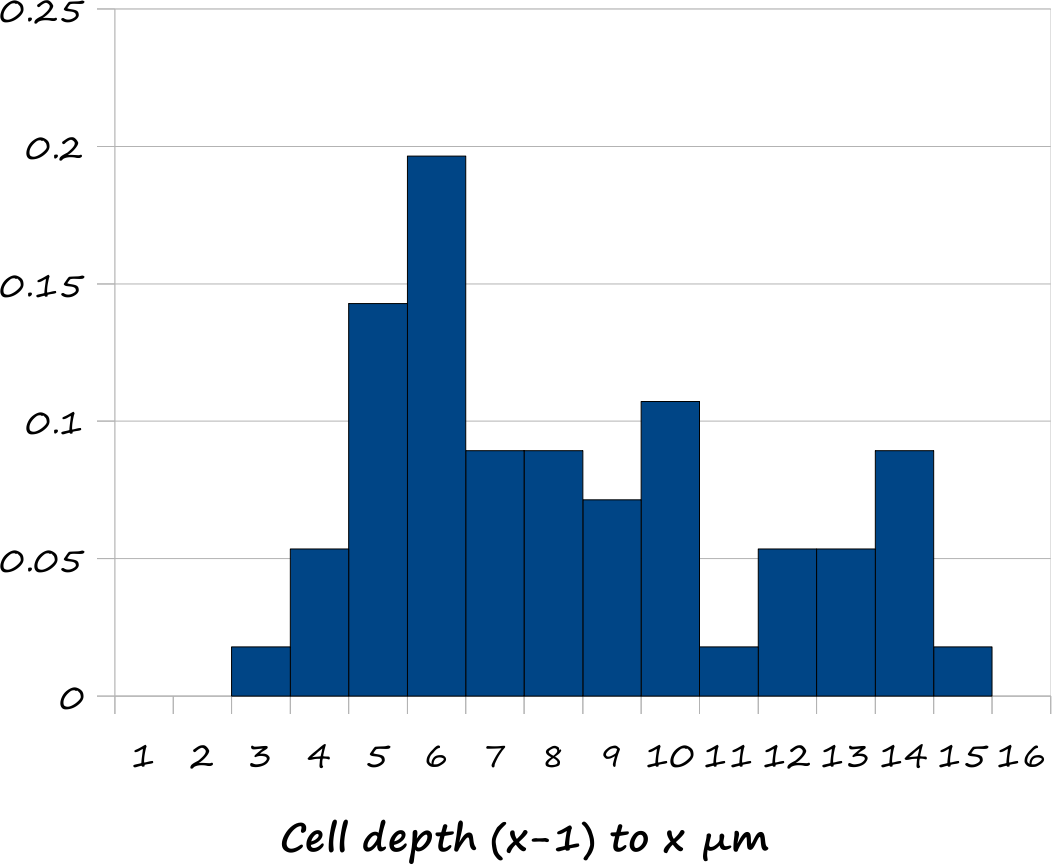
\includegraphics[width=3in]{consistency-cell-depth-distribution.png}
	\end{center}
	%\label{fig:cell-depth-distribution}
\end{figure}

In flat mounts, i.e.\ in the AP/DV plane, it is possible to measure the \textbf{mitotic index} as the number of PH3+ cells per unit area $m_d$. If PH3 only stains for a period of time $\tau_\textrm{mitosis}$, we may calculate the division rate as $$\lambda_d = \frac{\rho_d}{\tau_\textrm{mitosis}}\frac{m_d s [DV]_d}{p_d},$$ where $\rho_d$ is the proportion of progenitor cells in domain $d$, e.g.\ from the preliminary data, $\rho_d \simeq 1$. In practice, we do not know $\tau_\textrm{mitosis}$, though it is should be a constant of time and space; however, it is conceivable that $\rho_d$ may change through changes in $\lambda$, $\gamma$, $r_1$ or $r_2$ (in fact, may be quite generally a functional on their values for all previous times). From the data so far, we can see the change in $\lambda_d \tau_\textrm{mitosis} / \rho_d$:

\begin{figure}[h]
	\begin{center}
		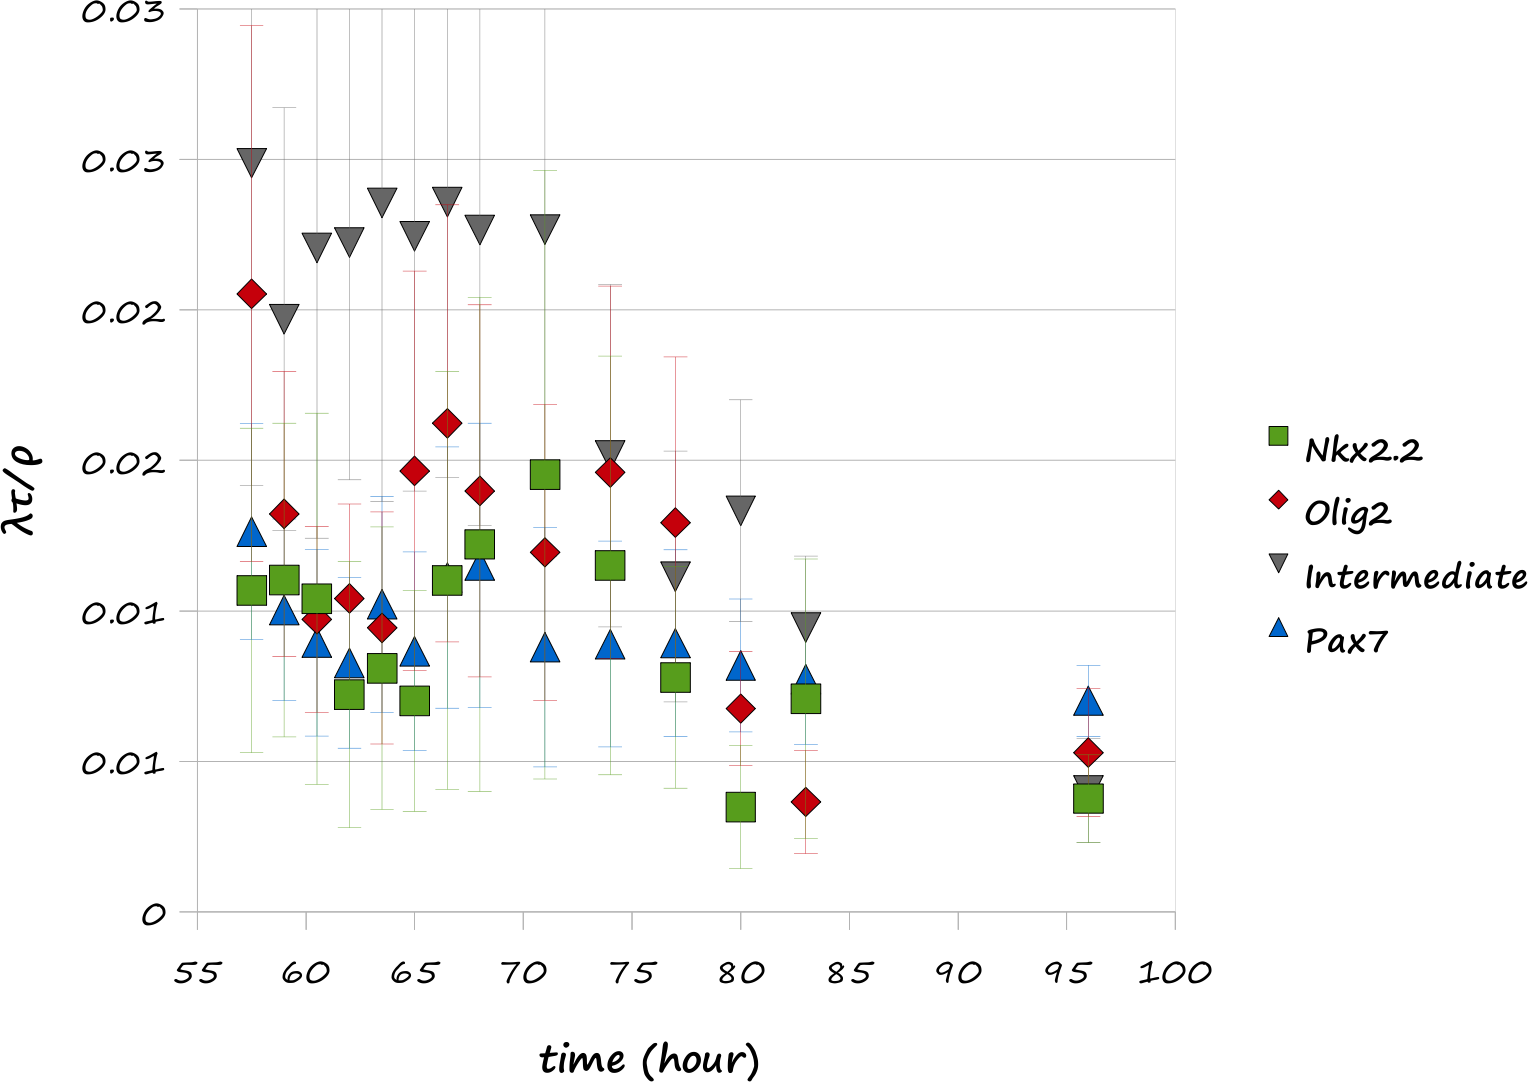
\includegraphics[width=4in]{consistency-mitotic-index.png}
	\end{center}
	%\label{fig:mitotic-index}
\end{figure}

\paragraph{Discussion}

Assuming a PH3 staining time $\tau_\textrm{mitosis} = \SI{15}{\minute}$ and $\rho_d = 1$ we find that a cell division time $1/\lambda_d \simeq \SI{25}{\hour}$, at least before $t \le \SI{75}{\hour}$. There is, however, a definite drop afterwards. The primary question is surely whether this is a decrease in division rate or a change of division ratios from favouring progenitor growth to favouring differentiation; of course, it could be both.

With a basic division process fixed, it is now feasible to consider clonal analysis. We expect full clonal size distributions will allow the mechanism by which growth occurs to be characterised.




\chapter{\label{ch:conclusion}Discussion and future work}


\newpage
\addcontentsline{toc}{chapter}{References}
\renewcommand\bibname{References}
%\bibliographystyle{apsrev}
\printbibliography[]

\end{document}
